% Generated fragments require trusted human review before compilation.
% This binder never requests shell escape or runs external tools.
\documentclass[11pt]{article}
% Trusted shared apparatus. Requires LuaLaTeX; never use shell escape.
\usepackage{fontspec}
\defaultfontfeatures{Ligatures=TeX}
\IfFontExistsTF{Noto Serif}{\setmainfont{Noto Serif}}{%
  \IfFontExistsTF{DejaVu Serif}{\setmainfont{DejaVu Serif}}{%
    \IfFontExistsTF{Times New Roman}{\setmainfont{Times New Roman}}{%
      \PackageError{gelfand-binder}{No configured Cyrillic serif font installed}{Install Noto Serif or DejaVu Serif, or select an installed Cyrillic font.}%
    }%
  }%
}
\IfFontExistsTF{Noto Sans}{\setsansfont{Noto Sans}}{%
  \IfFontExistsTF{DejaVu Sans}{\setsansfont{DejaVu Sans}}{\setsansfont{Arial}}%
}
\IfFontExistsTF{Noto Sans Mono}{\setmonofont{Noto Sans Mono}}{%
  \IfFontExistsTF{DejaVu Sans Mono}{\setmonofont{DejaVu Sans Mono}}{\setmonofont{Courier New}}%
}
\usepackage[a4paper,margin=22mm]{geometry}
\usepackage{amsmath,amssymb,amsthm,mathtools}
\usepackage{xcolor}
\usepackage{tikz}
\usepackage{tikz-cd}
\usetikzlibrary{arrows.meta,positioning,calc}
\usepackage{hyperref}
\hypersetup{unicode=true,colorlinks=true,linkcolor=blue,pdftitle={Gelfand transcription binder}}
\newtheorem{theorem}{Theorem}
\newtheorem{lemma}{Lemma}
\newtheorem{proposition}{Proposition}
\newtheorem{corollary}{Corollary}
\theoremstyle{definition}
\newtheorem{definition}{Definition}
\newtheorem{example}{Example}
\theoremstyle{remark}
\newtheorem{remark}{Remark}
\setlength{\parindent}{0pt}
\setlength{\parskip}{0.55em}
\setlength{\emergencystretch}{3em}
\newcommand{\SourcePage}[2]{%
  \clearpage\phantomsection\label{#1:source-page}%
  \addcontentsline{toc}{subsection}{#1}%
  {\small\sffamily\color{blue!60!black}Source scan frame: #1; visible page/leaf label: #2}\par\medskip%
}
\newcommand{\Unclear}[3]{%
  \begingroup\color{orange!70!black}%
  [Unresolved reading #1/#2: #3]\endgroup%
}
\newcommand{\Incomplete}[3]{%
  \par\begingroup\color{red!65!black}\textbf{Incomplete #1/#2:} #3\endgroup\par%
}
\newcommand{\SourceFigure}[3]{%
  \par\begingroup\color{blue!60!black}\textbf{\hyperref[#1:source-page]{Source figure #1/#2}:} #3%
  \par\textit{Consult the authoritative scan at this locator.}\endgroup\par%
}



% Reader layout only. Original diplomatic text is retained verbatim.
\setlength{\parskip}{0.35em}
\setlength{\emergencystretch}{4em}
\renewcommand{\SourcePage}[2]{%
  \par\addvspace{1em}\phantomsection\label{#1:source-page}%
  \addcontentsline{toc}{subsection}{#1}%
  {\footnotesize\sffamily\color{blue!55!black}#1%
    \def\givenlabel{#2}\def\nolabel{unlabelled}%
    \ifx\givenlabel\nolabel\else\quad[номер в источнике: #2]\fi
  }\par\nobreak\smallskip%
}
\renewcommand{\Unclear}[3]{%
  \begingroup\color{orange!65!black}%
  \ifmmode\text{[неясно: #3]}\else[неясно: #3]\fi\endgroup%
}
\renewcommand{\Incomplete}[3]{%
  \par\begingroup\color{red!60!black}\textbf{Неразобранный фрагмент:} #3%
  \endgroup\par%
}
\renewcommand{\SourceFigure}[3]{%
  \par\begingroup\color{blue!55!black}\textbf{Рисунок:} #3%
  \par{\small\textit{Исходный рисунок: \hyperref[#1:source-page]{#1}, #2.}}%
  \endgroup\par%
}
\hypersetup{pdftitle={Семинар И. М. Гельфанда. Дипломатическая транскрипция},pdfauthor={},pdfsubject={Русское рабочее издание с отмеченными сомнительными чтениями}}

\usepackage[normalem]{ulem}
\usepackage{newunicodechar}
\usepackage{adjustbox}
\newfontfamily\SourceSymbolFont{Segoe UI Symbol}
\newfontfamily\SourceCJKFont{MS Gothic}
\let\DiplomaticMathUnderline\underline
\renewcommand{\underline}[1]{\ifmmode\DiplomaticMathUnderline{#1}\else\uline{#1}\fi}
\newunicodechar{→}{\ifmmode\text{{\SourceSymbolFont\char"2192}}\else{\SourceSymbolFont\char"2192}\fi}
\newunicodechar{⇒}{\ifmmode\text{{\SourceSymbolFont\char"21D2}}\else{\SourceSymbolFont\char"21D2}\fi}
\newunicodechar{∀}{\ifmmode\text{{\SourceSymbolFont\char"2200}}\else{\SourceSymbolFont\char"2200}\fi}
\newunicodechar{∂}{\ifmmode\text{{\SourceSymbolFont\char"2202}}\else{\SourceSymbolFont\char"2202}\fi}
\newunicodechar{∈}{\ifmmode\text{{\SourceSymbolFont\char"2208}}\else{\SourceSymbolFont\char"2208}\fi}
\newunicodechar{∌}{\ifmmode\text{{\SourceSymbolFont\char"220C}}\else{\SourceSymbolFont\char"220C}\fi}
\newunicodechar{√}{\ifmmode\text{{\SourceSymbolFont\char"221A}}\else{\SourceSymbolFont\char"221A}\fi}
\newunicodechar{∞}{\ifmmode\text{{\SourceSymbolFont\char"221E}}\else{\SourceSymbolFont\char"221E}\fi}
\newunicodechar{∧}{\ifmmode\text{{\SourceSymbolFont\char"2227}}\else{\SourceSymbolFont\char"2227}\fi}
\newunicodechar{∩}{\ifmmode\text{{\SourceSymbolFont\char"2229}}\else{\SourceSymbolFont\char"2229}\fi}
\newunicodechar{∪}{\ifmmode\text{{\SourceSymbolFont\char"222A}}\else{\SourceSymbolFont\char"222A}\fi}
\newunicodechar{∫}{\ifmmode\text{{\SourceSymbolFont\char"222B}}\else{\SourceSymbolFont\char"222B}\fi}
\newunicodechar{∴}{\ifmmode\text{{\SourceSymbolFont\char"2234}}\else{\SourceSymbolFont\char"2234}\fi}
\newunicodechar{∼}{\ifmmode\text{{\SourceSymbolFont\char"223C}}\else{\SourceSymbolFont\char"223C}\fi}
\newunicodechar{≈}{\ifmmode\text{{\SourceSymbolFont\char"2248}}\else{\SourceSymbolFont\char"2248}\fi}
\newunicodechar{≠}{\ifmmode\text{{\SourceSymbolFont\char"2260}}\else{\SourceSymbolFont\char"2260}\fi}
\newunicodechar{≤}{\ifmmode\text{{\SourceSymbolFont\char"2264}}\else{\SourceSymbolFont\char"2264}\fi}
\newunicodechar{≥}{\ifmmode\text{{\SourceSymbolFont\char"2265}}\else{\SourceSymbolFont\char"2265}\fi}
\newunicodechar{⊕}{\ifmmode\text{{\SourceSymbolFont\char"2295}}\else{\SourceSymbolFont\char"2295}\fi}
\newunicodechar{⊗}{\ifmmode\text{{\SourceSymbolFont\char"2297}}\else{\SourceSymbolFont\char"2297}\fi}
\newunicodechar{①}{\ifmmode\text{{\SourceSymbolFont\char"2460}}\else{\SourceSymbolFont\char"2460}\fi}
\newunicodechar{②}{\ifmmode\text{{\SourceSymbolFont\char"2461}}\else{\SourceSymbolFont\char"2461}\fi}
\newunicodechar{③}{\ifmmode\text{{\SourceSymbolFont\char"2462}}\else{\SourceSymbolFont\char"2462}\fi}
\newunicodechar{④}{\ifmmode\text{{\SourceSymbolFont\char"2463}}\else{\SourceSymbolFont\char"2463}\fi}
\newunicodechar{Ⓗ}{\ifmmode\text{{\SourceSymbolFont\char"24BD}}\else{\SourceSymbolFont\char"24BD}\fi}
\newunicodechar{〃}{\ifmmode\text{{\SourceCJKFont\char"3003}}\else{\SourceCJKFont\char"3003}\fi}


% Reader revision 3. Annotation wording and candidates remain unchanged.
\setmainfont{NotoSerif-Regular.ttf}[Path=C:/Windows/Fonts/,ItalicFont=NotoSerif-Italic.ttf,BoldFont=NotoSerif-Bold.ttf,BoldItalicFont=NotoSerif-BoldItalic.ttf]
\usetikzlibrary{shapes.geometric,decorations.pathreplacing,decorations.markings,patterns,fit}
\newsavebox{\ReaderAnnotationBox}
\newcommand{\ReaderAnnotation}[1]{%
  \sbox{\ReaderAnnotationBox}{[неясно: #1]}%
  \ifdim\wd\ReaderAnnotationBox>.70\linewidth
    \parbox[t]{.70\linewidth}{\raggedright[неясно: #1]}%
  \else\usebox{\ReaderAnnotationBox}\fi%
}
\ExplSyntaxOn
\cs_new_protected:Npn \reader_unclear_candidate:n #1
 {
  \tl_set:Nx \l_tmpa_tl { \tl_to_str:n {#1} }
  % Text explicitly guarded inside a mathematical candidate remains math-safe.
  \regex_replace_all:nnN { \\(?:text|textrm|textnormal|textbf|operatorname)\s*\{[^{}]*\} } { } \l_tmpa_tl
  \regex_match:nVTF { [\x{0400}-\x{052F}] | \$ } \l_tmpa_tl
   { \ifmmode \text{\ReaderAnnotation{#1}} \else \ReaderAnnotation{#1} \fi }
   {
    \ifmmode
      [\text{неясно:~}#1]
    \else
      \regex_match:nVTF { [_^] | \\ } \l_tmpa_tl
       { \ensuremath{[\text{неясно:~}#1]} }
       { \ReaderAnnotation{#1} }
    \fi
   }
 }
\RenewDocumentCommand \Unclear { m m m }
 { \begingroup\color{orange!65!black}\reader_unclear_candidate:n{#3}\endgroup }
\ExplSyntaxOff
\newsavebox{\ReaderIncompleteBox}
\newcommand{\ReaderIncompleteNote}[1]{%
 \sbox{\ReaderIncompleteBox}{\textbf{Неразобранный фрагмент:} #1}%
 \ifdim\wd\ReaderIncompleteBox>.70\linewidth
  \parbox[t]{.70\linewidth}{\raggedright\textbf{Неразобранный фрагмент:} #1}%
 \else\usebox{\ReaderIncompleteBox}\fi%
}
\renewcommand{\Incomplete}[3]{%
 \ifmmode\text{\color{red!60!black}\ReaderIncompleteNote{#3}}%
 \else\leavevmode\begingroup\color{red!60!black}\ReaderIncompleteNote{#3}\endgroup\fi%
}
% Ragged right avoids stretching long untranslated abbreviations into margins.
\AtBeginDocument{\raggedright}
\newunicodechar{А}{\ifmmode\text{\char"410\relax}\else\char"410\relax\fi}
\newunicodechar{Б}{\ifmmode\text{\char"411\relax}\else\char"411\relax\fi}
\newunicodechar{В}{\ifmmode\text{\char"412\relax}\else\char"412\relax\fi}
\newunicodechar{Г}{\ifmmode\text{\char"413\relax}\else\char"413\relax\fi}
\newunicodechar{Д}{\ifmmode\text{\char"414\relax}\else\char"414\relax\fi}
\newunicodechar{Е}{\ifmmode\text{\char"415\relax}\else\char"415\relax\fi}
\newunicodechar{Ж}{\ifmmode\text{\char"416\relax}\else\char"416\relax\fi}
\newunicodechar{З}{\ifmmode\text{\char"417\relax}\else\char"417\relax\fi}
\newunicodechar{И}{\ifmmode\text{\char"418\relax}\else\char"418\relax\fi}
\newunicodechar{Й}{\ifmmode\text{\char"419\relax}\else\char"419\relax\fi}
\newunicodechar{К}{\ifmmode\text{\char"41A\relax}\else\char"41A\relax\fi}
\newunicodechar{Л}{\ifmmode\text{\char"41B\relax}\else\char"41B\relax\fi}
\newunicodechar{М}{\ifmmode\text{\char"41C\relax}\else\char"41C\relax\fi}
\newunicodechar{Н}{\ifmmode\text{\char"41D\relax}\else\char"41D\relax\fi}
\newunicodechar{О}{\ifmmode\text{\char"41E\relax}\else\char"41E\relax\fi}
\newunicodechar{П}{\ifmmode\text{\char"41F\relax}\else\char"41F\relax\fi}
\newunicodechar{Р}{\ifmmode\text{\char"420\relax}\else\char"420\relax\fi}
\newunicodechar{С}{\ifmmode\text{\char"421\relax}\else\char"421\relax\fi}
\newunicodechar{Т}{\ifmmode\text{\char"422\relax}\else\char"422\relax\fi}
\newunicodechar{У}{\ifmmode\text{\char"423\relax}\else\char"423\relax\fi}
\newunicodechar{Ф}{\ifmmode\text{\char"424\relax}\else\char"424\relax\fi}
\newunicodechar{Х}{\ifmmode\text{\char"425\relax}\else\char"425\relax\fi}
\newunicodechar{Ц}{\ifmmode\text{\char"426\relax}\else\char"426\relax\fi}
\newunicodechar{Ч}{\ifmmode\text{\char"427\relax}\else\char"427\relax\fi}
\newunicodechar{Ш}{\ifmmode\text{\char"428\relax}\else\char"428\relax\fi}
\newunicodechar{Щ}{\ifmmode\text{\char"429\relax}\else\char"429\relax\fi}
\newunicodechar{Ъ}{\ifmmode\text{\char"42A\relax}\else\char"42A\relax\fi}
\newunicodechar{Ы}{\ifmmode\text{\char"42B\relax}\else\char"42B\relax\fi}
\newunicodechar{Ь}{\ifmmode\text{\char"42C\relax}\else\char"42C\relax\fi}
\newunicodechar{Э}{\ifmmode\text{\char"42D\relax}\else\char"42D\relax\fi}
\newunicodechar{Ю}{\ifmmode\text{\char"42E\relax}\else\char"42E\relax\fi}
\newunicodechar{Я}{\ifmmode\text{\char"42F\relax}\else\char"42F\relax\fi}
\newunicodechar{а}{\ifmmode\text{\char"430\relax}\else\char"430\relax\fi}
\newunicodechar{б}{\ifmmode\text{\char"431\relax}\else\char"431\relax\fi}
\newunicodechar{в}{\ifmmode\text{\char"432\relax}\else\char"432\relax\fi}
\newunicodechar{г}{\ifmmode\text{\char"433\relax}\else\char"433\relax\fi}
\newunicodechar{д}{\ifmmode\text{\char"434\relax}\else\char"434\relax\fi}
\newunicodechar{е}{\ifmmode\text{\char"435\relax}\else\char"435\relax\fi}
\newunicodechar{ж}{\ifmmode\text{\char"436\relax}\else\char"436\relax\fi}
\newunicodechar{з}{\ifmmode\text{\char"437\relax}\else\char"437\relax\fi}
\newunicodechar{и}{\ifmmode\text{\char"438\relax}\else\char"438\relax\fi}
\newunicodechar{й}{\ifmmode\text{\char"439\relax}\else\char"439\relax\fi}
\newunicodechar{к}{\ifmmode\text{\char"43A\relax}\else\char"43A\relax\fi}
\newunicodechar{л}{\ifmmode\text{\char"43B\relax}\else\char"43B\relax\fi}
\newunicodechar{м}{\ifmmode\text{\char"43C\relax}\else\char"43C\relax\fi}
\newunicodechar{н}{\ifmmode\text{\char"43D\relax}\else\char"43D\relax\fi}
\newunicodechar{о}{\ifmmode\text{\char"43E\relax}\else\char"43E\relax\fi}
\newunicodechar{п}{\ifmmode\text{\char"43F\relax}\else\char"43F\relax\fi}
\newunicodechar{р}{\ifmmode\text{\char"440\relax}\else\char"440\relax\fi}
\newunicodechar{с}{\ifmmode\text{\char"441\relax}\else\char"441\relax\fi}
\newunicodechar{т}{\ifmmode\text{\char"442\relax}\else\char"442\relax\fi}
\newunicodechar{у}{\ifmmode\text{\char"443\relax}\else\char"443\relax\fi}
\newunicodechar{ф}{\ifmmode\text{\char"444\relax}\else\char"444\relax\fi}
\newunicodechar{х}{\ifmmode\text{\char"445\relax}\else\char"445\relax\fi}
\newunicodechar{ц}{\ifmmode\text{\char"446\relax}\else\char"446\relax\fi}
\newunicodechar{ч}{\ifmmode\text{\char"447\relax}\else\char"447\relax\fi}
\newunicodechar{ш}{\ifmmode\text{\char"448\relax}\else\char"448\relax\fi}
\newunicodechar{щ}{\ifmmode\text{\char"449\relax}\else\char"449\relax\fi}
\newunicodechar{ъ}{\ifmmode\text{\char"44A\relax}\else\char"44A\relax\fi}
\newunicodechar{ы}{\ifmmode\text{\char"44B\relax}\else\char"44B\relax\fi}
\newunicodechar{ь}{\ifmmode\text{\char"44C\relax}\else\char"44C\relax\fi}
\newunicodechar{э}{\ifmmode\text{\char"44D\relax}\else\char"44D\relax\fi}
\newunicodechar{ю}{\ifmmode\text{\char"44E\relax}\else\char"44E\relax\fi}
\newunicodechar{я}{\ifmmode\text{\char"44F\relax}\else\char"44F\relax\fi}
\newunicodechar{Ё}{\ifmmode\text{\char"401\relax}\else\char"401\relax\fi}
\newunicodechar{ё}{\ifmmode\text{\char"451\relax}\else\char"451\relax\fi}

\newunicodechar{æ}{\ifmmode\text{\char"E6\relax}\else\char"E6\relax\fi}
\newunicodechar{−}{\ifmmode\mathbin{\text{\SourceSymbolFont\char"2212\relax}}\else{\SourceSymbolFont\char"2212\relax}\fi}


% Reader-only pairing support; accepted raw bodies remain unchanged.
\RequirePackage{graphicx}
\RequirePackage{adjustbox}
\newcommand{\ReaderOriginalPanel}[2]{%
  \begin{minipage}[t]{.48\linewidth}\vspace{0pt}\centering
    \includegraphics[width=\linewidth,keepaspectratio]{#1}\par\smallskip
    {\scriptsize Оригинал рукописного рисунка: #2}\par
  \end{minipage}%
}
\newcommand{\ReaderDiagramPair}[3]{%
  \par\noindent\begingroup
  \ReaderOriginalPanel{#1}{#2}\hfill
  \begin{minipage}[t]{.48\linewidth}\vspace{0pt}\centering
    {\scriptsize Типографское воссоздание}\par\smallskip
    \begin{adjustbox}{max width=\linewidth}#3\end{adjustbox}\par
  \end{minipage}%
  \endgroup\par\smallskip
}
\newcommand{\ReaderDescriptionPair}[3]{%
  \par\noindent\begingroup
  \ReaderOriginalPanel{#1}{#2}\hfill
  \begin{minipage}[t]{.48\linewidth}\vspace{0pt}\raggedright
    {\scriptsize Типографское описание}\par\smallskip
    #3\par
  \end{minipage}%
  \endgroup\par\smallskip
}


\begin{document}
\begin{center}
{\Large Семинар И. М. Гельфанда}\par\medskip
{\LARGE Дипломатическая транскрипция}\par\bigskip
{\large Рабочее русское издание}\par\medskip
{\large Том 08 из 34. Архивная глава 008}\par\bigskip
Кадры GELFAND-P000554 -- GELFAND-P000602\par
\end{center}
\medskip
Сокращения, отменённые записи и сомнительные чтения сохранены.
Неразобранные фрагменты отмечены в тексте. Математические утверждения
источника переданы без молчаливых исправлений.

В текущем комплекте приняты 165 из 165 возвратов; учтены 1527 из 1527 кадров. Кадров без принятого возврата: 0.
Статусы кадров в отчётах о полноте: транскрибированы 1168, неразборчивы 357, частично прочитаны 1, недоступны 1.
Нерешённых записей журнала чтений: 6820.
Статус «неразборчивый» может отмечать локальную утрату зачёркнутой записи;
он не означает отсутствия всего кадра.
Сверка с рукописью продолжается. Рабочие журналы чтений и происхождения
данных сохранены отдельно.

Ограничения исходного комплекта: повреждённый исходный скан GELFAND-P000722; каталожные записи 603, 694 без сканов; в архивной главе 029 не перечислена часть 25.

Границы кадров показаны небольшими синими указателями; печатный текст
продолжается без обязательного разрыва страницы после каждого кадра.
\bigskip\hrule\bigskip
\SourcePage{GELFAND-P000554}{unlabelled}
\underline{2/IX−74. Сем. Гельфанда} (32-й год работы семинара)
\underline{Джусти.}
1. Singularities and regularity
\Unclear{GELFAND-P000554}{title-old}{Между Singularities и and небольшой плотный переписанный знак; прежние штрихи не установлены.}
of solutions of non-linear elliptic (and parabolic) systems.
\Unclear{GELFAND-P000554}{line-prefix-old}{Перед of solutions два плотных вертикальных и косых штриха; старый короткий знак не установлен.}
Nash, De giorgi, Moser. — Regularity: 1 equation linear with
\Unclear{GELFAND-P000554}{linear-old}{После linear перед with зачёркнута короткая группа; предположительно di…t или dif, отдельные буквы не установлены. Полное слово не дописано.}
discont. coeff. (Höld. coeff.) $\Rightarrow$ regul. for non linear with smooth coeff.
\underline{Systems} — неверно.
\Unclear{GELFAND-P000554}{systems-old}{После тире перед «неверно» короткий перечёркнутый знак с горизонтальным выходом справа; старое чтение не установлено.}
Быв. ср. коэфф. и несгр. решения
\Unclear{GELFAND-P000554}{systems-caption}{Начальные сокращения перед «коэфф.» и перед «решения» читаются предположительно как «Быв. ср.» и «несгр.»; развёрнутые слова не введены.}
1968 Miranda, Giusti — сист. с аналит. коэфф. с разр. решениями
\Unclear{GELFAND-P000554}{giusti-name}{В начале Giusti плотные переписанные штрихи; текущая фамилия передана предположительно, старые буквы не установлены.}
\begin{gather*}
\Sigma\text{ — singular set.}\\
(1)\quad\Sigma\text{ closed}\\
(2)\quad\dim\Sigma<n-2
\end{gather*}

2. Boundary value problems for surfaces of prescribed mean curvature.
$u:\Omega\to\mathbb R$,\quad graph $u=S$.
\begin{adjustbox}{max width=\linewidth}
\begin{tikzpicture}
\draw (0,0) .. controls (-0.6,0.3) and (-0.4,1.2) .. (0.2,1.4) .. controls (0.9,1.5) and (1.1,0.7) .. (0.9,0.1) .. controls (0.6,-0.1) and (0.2,-0.1) .. (0,0);
\draw (3,0)--(4.8,0);\node at (3.9,-0.3) {$\Omega$};
\draw (3.2,0.15)--(3.2,1.3);\draw (5,0.15)--(5,1.3);
\draw (3.2,1.3) .. controls (3.9,1.7) and (3.9,0.9) .. (4.4,1.05) .. controls (4.6,1.1) and (4.8,1.2) .. (5,1.2);
\end{tikzpicture}
\end{adjustbox}
\begin{equation*}
H(x)=\frac1n\sum\frac{\partial}{\partial x_i}
\left(\frac{\partial u/\partial x_i}{\sqrt{1+|grad\,u|^2}}\right)
\end{equation*}
$H$ не очень велико (иначе неразрешимо). Зависит от геометрии области, ф-и $H(x)$ и т. д.
Это и будет в следующий раз.

\underline{С. П. Новиков.} (и Дубровин).
Абелево мн-зие $\xi_1,\ldots,\xi_{2n}$ — базис в $\mathbb C^n$ (над $\mathbb R$),
$T^{2n}$ — соотв. тор. Пусть абелево мн-зие (алгебраич. мн-зие).
Как описать все торы?
$n=2$ уже нетривиально.
\begin{equation*}
y^2=P_{2n+1}(x)\qquad\text{рим. поверхность}\quad\Rightarrow\quad\text{тор.}
\end{equation*}
\Unclear{GELFAND-P000554}{cohomology-old}{Перед H¹ зачёркнуто короткое написание: начало похоже на «Вид…», справа в-подобная петля. Эти фрагменты переданы предположительно, связное чтение не установлено.}
\begin{gather*}
R\longrightarrow J^{2n}(R).\quad(\text{тор})\\
\underbrace{H^1(R,\mathbb C)/H^1(R,\mathbb Z)}_{\text{тор такой}}\\
k=0,\ldots,n-1,\qquad\omega_k=\frac{x^k\,dx}{\sqrt{P_{2n+1}(x)}}
\end{gather*}
$\leftarrow$ всюду регулярные дифференциалы.
Базис — формы $\omega_k$.
\begin{equation*}
P_{2n+1}(x)=\prod(x-x_\alpha).
\end{equation*}
Всё опр. набором корней.
\SourceFigure{GELFAND-P000554}{moduli-maps}{Внизу слева две схемы: верхняя M с шапкой направлена вправо к M, затем стрелка с R над ней к B. Ниже M с двумя верхними знаками направлена вправо к M с волнистым верхним знаком; от неё наклонная стрелка вправо вверх и справа J(R). Точное различение всех шапок и волн и конец второй стрелки не установлены.}
$M$ — совок. рим. поверхностей
$B$ — верхняя полуплоскость Зигеля
(накрытие мн-зия модулей).
по набору корней строится многочлен, а по нему тор.

\SourcePage{GELFAND-P000555}{unlabelled}
\begin{gather*}
p_1,p_2,q_1,q_2,c,d.\qquad\mathbb C^6\text{ или }\mathbb C^4_{c,d}\\
J_1=p_1p_2+V(q_1,q_2)\\
J_2=p_1^2-2q_1p_1p_2+2(q_2-c)p_2^2+D(q_1,q_2)\\
\Omega=\sum_{\alpha=1}^2dp_\alpha\wedge dq_\alpha.\\
\langle J_1,J_2\rangle\equiv0.
\end{gather*}
ск. Пуассона.
\begin{equation*}
V=-\left(\frac{q_2^2}{2}+\frac52q_1^2q_2+\frac52q_1^4\right)+c_1q_1^2-d_1q_1
\end{equation*}
\Unclear{GELFAND-P000555}{potential-symbol}{Перед равенством плотный знак с V-подобными верхними ветвями и чёрной левой нижней частью; V передано предположительно, прежние штрихи не установлены.}
\begin{equation*}
D=q_1^5+2c_1q_1^3+d_1q_1^2-4q_1q_2^2+4c_1q_1q_2-2d_1q_2.
\end{equation*}
\begin{equation*}
[X_{J_1},X_{J_2}]=0.
\end{equation*}
Получ. 2 коммут. поля.
Соотв. орбиты — абелево мн-зие
\begin{gather*}
J_1=const\\J_2=const
\end{gather*}
\Unclear{GELFAND-P000555}{orbit-old}{Слева перед двумя равенствами перечёркнута короткая старая группа знаков, похожая на J с индексом; индекс и остальные штрихи не установлены.}
[Два равенства объединены скобкой: тор.]
\underline{Следствие.} совок. всех их — унирац. многообразие.
\begin{equation*}
R:\quad y^2=x^5+\frac{c_1}{4}x^3-\frac{d_1}{16}x^2+
\left(\frac{J_1}{32}+\frac{c_1^2}{4}\right)x+\frac{J_2}{2^8}+\frac{c_1d_1}{2^7}
\end{equation*}
$R$ — рим. пов., $S^nR$ — симметр. степень $R$
$(J_1,\ldots,J_n)$ и симметризация.
\begin{gather*}
S^nR\longrightarrow J(R).\\
(P_1,\ldots,P_n)\overset A\longrightarrow(\alpha_1,\ldots,\alpha_n)
\end{gather*}
отобр. Абеля. (Теор. Абеля — это изоморфизм).
\SourceFigure{GELFAND-P000555}{abel-paths}{Слева точка Q и две кривые к точкам P1 наверху и Pn справа; начало верхней кривой и стрелочные признаки не различены уверенно. Видимые подписи Q, P1, Pn сохранены в описании.}
\begin{equation*}
(P_1,\ldots,P_n)\longrightarrow
\left(\sum_{k=1}^n\int_Q^{P_k}\omega_s\right)
\end{equation*}
[Под скобкой: $\alpha_s$.]
\begin{gather*}
L=-\frac{d^2}{dx^2}+u(x),\\
u(x+T)=u(x)\text{ или квазипериодичн.}\\
\text{Соб. ф-я }L\Psi(x,E)=E\Psi,\\
\Psi(x+T)=\lambda\Psi(x),\qquad|\lambda|=1,\qquad\lambda=e^{ip(E)}
\end{gather*}
(Блоховские соб. ф-и)
Для почти периодичн. ансамбль таких соб. ф-й не обр. полную систему.
\Incomplete{GELFAND-P000555}{almost-periodic-old}{После «периодичн.» плотный зачёркнутый короткий фрагмент целиком не восстановлен.}
\begin{equation*}
\Psi|_{x_0}=1\text{ — нормировка}
\end{equation*}
$\Psi(x,E,x_0)$\qquad$(\Psi,\overline\Psi)$ — 2 соб. ф-и.
по $E$ ветвится в концах отр. спектра. Получ. рим. пов. беск. рода.
2 листа, т. к. 2 соб. ф-и.

\SourcePage{GELFAND-P000556}{unlabelled}
Мн-во потенц. с зад. зонной структурой — мн-зие Якоби этой рим. поверхности (есть ф-ии).
\Unclear{GELFAND-P000556}{zonal-overwrite}{В слове «зонной» первые средние штрихи перечёркнуты и переписаны; текущая форма читается, прежние буквы не установлены.}
\SourceFigure{GELFAND-P000556}{spectrum-line}{Горизонтальная спектральная линия: утолщённый участок от x1 к x2, затем тонкий промежуток и ещё утолщённый участок с концами без подписей; правее после тонкого промежутка утолщённый луч от x2n+1. Подписи x1, x2, x2n+1 и «спектр.» видны; точное число не подписанных промежуточных концов не установлено.}
Потенц. с зад. зонной структурой — соотв. тор (мн-зие Якоби).

\underline{9/IX−74. Сем. Гельфанда.}
\underline{Бесага} (Варшава). $Z$-множества Андерсона и их приложения.
(R. D. Anderson)
$X$ — полное метриз. пр-во. $A\subset X$, $\overline A=A$.
$A$ наз. $Z$-мн-вом, если $\forall$ непр. отобр. $f:I^\infty\to X$,
$\forall\varepsilon>0$, $\exists g:I^\infty\to X\setminus A$, $\rho(f,g)<\varepsilon$.
[Под $I^\infty$: гильб. куб.]
\begin{equation*}
Q=[-1,1]^\infty,\qquad P=(-1,1)^\infty.\qquad(Q\setminus P)\text{ — }Z\text{-мн-во}
\end{equation*}
\underline{Св-ва:} $1^{\circ}$ Если $A,B$ — $Z$-мн-ва (в $Q$), то $f:A\cong B$ продолж. до
гомеом. всего пр-ва.
\Unclear{GELFAND-P000556}{property-number}{Номер первого свойства и кружок переписаны плотнее; 1° передано предположительно, более ранние штрихи не установлены.}
\Unclear{GELFAND-P000556}{extension-old}{Перед «гомеом.» зачёркнуто короткое написание, предположительно «гомео»; конечные переплетённые буквы не установлены и сокращение не развёрнуто.}
$Z_\sigma$-мн-во — счётное объед. $Z$-мн-в.
$2^{\circ}$ Сущ. максимальное $Z_\sigma$-мн-во
\underline{Гельфанд.}
Рассм. $\mathbb R^\infty$ в тих. топологии и пр-во $S$ лучей, вых. из 0
в ест. топологии. Док., что на $S$ любая непр. ф-я $const$
\Incomplete{GELFAND-P000556}{rays-old}{Между «лучей» и «вых.» плотный перечёркнутый фрагмент целиком не восстановлен.}
\Unclear{GELFAND-P000556}{constant-old}{Перед const небольшой чёрный переписанный знак с короткими краевыми штрихами; прежний знак не установлен.}
(Гельф., Фукс. Функц. анализ I, 4).
\underline{Бесага.} Все сепараб. пр-ва Фреше гомеоморфны.

\underline{Джусти.} $\Omega\subset\mathbb R^n$
[Слева от системы уравнений: отдельный замкнутый неровный овальный контур без подписи; внутри пять косых штрихов.]
\begin{equation*}
\left\{\begin{aligned}
\sum_{i=1}^nD_i\left\{\frac{D_i u}{\sqrt{1+|Du|^2}}\right\}&=-H(x,u)\quad\text{в }\Omega,\\
u&=\Phi\quad\text{на }\partial\Omega.
\end{aligned}\right.
\qquad D_i=\frac\partial{\partial x_i}.
\end{equation*}
$n$-кр. средн. кривизна = лев. часть ур-я
$H\equiv0\quad\Rightarrow\quad minimal\ surface$.
\SourceFigure{GELFAND-P000556}{graph-cylinder}{Слева вертикальные стороны над основанием Ω и волнистая линия между ними; внутри отдельный вертикальный штрих от волнистой линии вниз к основанию с небольшим нижним стрелочным знаком. Точная связь этого штриха с изображённой поверхностью не установлена.}
\underline{Example 1.}\quad$\Omega$, $n=2$, $H=0$.
\SourceFigure{GELFAND-P000556}{annulus}{Справа circular annulus: наружный овал, внутренний круг и косая штриховка между ними; внутри малые подписи 1 и 2 с радиальным штрихом, точная привязка обеих подписей к окружностям не установлена.}
circular annulus.
\begin{equation*}
\Phi=\begin{cases}0&|x|=2\\M&|x|=1\end{cases}
\end{equation*}
Solution: $u(r)$, $r=|x|$.
\Unclear{GELFAND-P000556}{radial-overwrites}{В Solution и в последующих формулах начальные u переписаны плотными петлями; текущие u переданы, прежние знаки не установлены.}
\begin{gather*}
u(r)=c\log\frac{2+\sqrt{4-c^2}}{r+\sqrt{r^2-c^2}},\qquad0\le c\le1,\\
u(1)=M\quad\Rightarrow\quad u(1)\le\log(2+\sqrt3)=M_0.
\end{gather*}

\SourcePage{GELFAND-P000557}{unlabelled}
При $M>M_0$ решений нет.
\underline{Экспер. проверка:} мыльн. пузырь осторожно поднимаем палку
steak.
\SourceFigure{GELFAND-P000557}{soap-surfaces}{Вверху три нумерованные схемы: 1) штрихованный овальный диск, справа от него отдельный короткий почти горизонтальный штрих без отчётливого наконечника, а под диском вертикальный стержень с косой штриховкой и верхней стрелкой; 2) небольшая расширяющаяся юбка вокруг двух вертикальных линий; 3) длинный стержень и широкая юбка. Ниже после «если провол. кольцо, то» отдельная поверхность с узкой шейкой, верхним овальным кольцом и широким овальным основанием. Пересечения, штриховка и отдельные контуры видны; точные пространственные склейки и размеры не установлены.}
если провол. кольцо, то
\underline{Example 2.}\quad$n=1$,\quad$\Omega=(-1,1)$
\begin{equation*}
u=3x^{1/3}
\end{equation*}
\Unclear{GELFAND-P000557}{cube-root-symbol}{Первый знак перед =3x имеет два плотных верхних штриха и нижнюю дугу; u передано предположительно, чтение H не исключено.}
\begin{equation*}
\left(\frac{u'}{\sqrt{1+u'^2}}\right)'=-\frac23x^{4/3}(1+x^{4/3})^{-3/2}
\end{equation*}
[Правая часть подчёркнута скобкой: непрер.]
\Unclear{GELFAND-P000557}{derivative-power}{Малый показатель первой степени x имеет крюк, вертикаль и нижнюю черту: 4/3 передано предположительно, чтение 1/3 не исключено. Во второй степени 4/3 читается яснее. Вычисленная степень 1/3 не подставлена вместо источника.}
$u$ — недифф.
\Unclear{GELFAND-P000557}{nondifferentiable-old}{Перед «u — недифф.» зачёркнуто короткое написание; предположительно «об…» с высокой петлёй, последние буквы не установлены.}
\begin{gather*}
u(-1)=-3,\qquad u(1)=3\\
\text{Пусть }u(-1)=3,\qquad u(1)=3+A\\
\frac{u'}{\sqrt{1+u'^2}}=(1+x^{4/3})^{-1/2}\\
u'\le x^{-2/3}\\
u(x)\le-3+\int_{-1}^xt^{-2/3}\,dt=3x^{1/3}
\end{gather*}
\begin{gather*}
\mathcal F(u)=\int_\Omega\sqrt{1+|Du|^2}\,dx+\int_\Omega\lambda(x,u)\,dx.\\
\lambda(x,t)=\int_0^tH(x,s)\,ds
\end{gather*}
Надо найти $min$.
При усл. $|u'|\le K$ есть $min$. (иначе нет).
$u_k$ — реш. Пусть $k\to+\infty$.\quad$u_k\to u_0$?
$u$ — Lip-contin. solut.\quad$A\subset\Omega$
\begin{gather*}
\int_AH(x)\,dx=\int_{\partial A}n_i\frac{D_i u}{\sqrt{1+|Du|^2}}\,dH_{n-1}\\
\left|\int_AH(x)\,dx\right|\le(1-\varepsilon_0)H_{n-1}(\partial A)\\
1-\varepsilon_0=\sup_\Omega\frac{|Du|}{\sqrt{1+|Du|^2}}.
\end{gather*}
[Последнее равенство в рамке.]
Поэтому $H$ не очень велико.

\SourcePage{GELFAND-P000558}{unlabelled}
\begin{equation*}
(1)\quad H^{1,1}=W_1^1\qquad
\mathcal F(u)=\int_\Omega\sqrt{1+|Du|^2}\,dx+\int_\Omega\lambda(x,u)\,dx+
\int_{\partial\Omega}|u-\Phi|\,dH_{n-1}.
\end{equation*}
$BV(\Omega)$ = $L^1$-ф-и, у к-рых 1-е произв. — меры (Радона).
\begin{equation*}
\text{т. е. }f\in BV\quad\Longleftrightarrow\quad f\in L^1,
\quad\sup\left\{\int_\Omega f\,div\,\vec g\,dx,\quad\vec g\in C_0^1(\Omega),\ |g|\le1\right\}<+\infty
\end{equation*}
\begin{equation*}
sup=\int_\Omega|Df|\,dx
\end{equation*}
\Unclear{GELFAND-P000558}{variation-bars}{В основном интеграле видны одиночные |Df|; над Df отдельно вписаны две вертикальные черты, слева от них перечёркнут короткий знак. Их прежнее чтение и точная связь со строкой не установлены.}
\underline{Площадь}\quad$\underline{f\in BV}$.
\begin{equation*}
A(f)=\int\sqrt{1+|Df|^2}\,dx
=\sup\left\{\int_\Omega(g_0+f\,div\,\vec g)\,dx,\quad g_0,g\in C_0^1,\quad g_0^2+|g|^2\le1\right\}.
\end{equation*}
[Под равенством после первого интеграла: def; на поле: area.]
$(Af)$ lower semicont. with respect to $L^1$.
\Unclear{GELFAND-P000558}{semicontinuity-old}{После L¹ зачёркнуто английское написание с предположительными остатками …nt…y. Видимые петли слева, t-подобные штрихи и нисходящий y-подобный конец допускают также continuity или cont…ty; эти чтения предположительны. Полное слово не установлено; зачёркивание сохранено, теория не служит доказательством букв.}
(2) Bounded sets in BV are relatively compact in $L_1$.

\underline{Дубровин.}
\begin{equation*}
L=-\frac{d^2}{dx^2}+u(x),\qquad u(x+T)=u(x)
\end{equation*}
$E$ — спектр. параметр.
\SourceFigure{GELFAND-P000558}{spectral-lines}{Две горизонтальные спектральные схемы: первая имеет два утолщённых конечных участка и правую стрелку с E; вторая подписана E1, E2, E2N+1 и заканчивается утолщённым лучом с наконечником вправо. Под подписью E1 видна отдельная малая незаполненная петля; её значение не установлено. Неподписанные промежуточные границы и точное соответствие линий не установлены.}
Иногда лакуны исчезают.
Пусть $u(x)$ — конечнозонный потенциал.
\begin{equation*}
R(E)=\prod(E-E_i)
\end{equation*}
Рассм. рим. пов. ф-и $\sqrt{R(E)}$ — обозн. $\Gamma_N$.
блоховские соб. ф-и аналит. прод. на $\Gamma_N\setminus\infty$
\Incomplete{GELFAND-P000558}{continuation-old}{Справа после утверждения об аналитическом продолжении старая скобочная запись покрыта частой косой штриховкой; целиком не восстановлена.}
(мероморфно).
$N$ — род.
и имеет $N$ полюсов и $N$ нулей.
блоховск. соб. ф-я: $\Psi(x,E,x_0)$
Полюса $\gamma_i(x_0)$.
есть естеств. проец.
\begin{equation*}
\Gamma_N\longrightarrow\mathbb C_E.
\end{equation*}
2-листн. накрытие.
\SourceFigure{GELFAND-P000558}{covering-ovals}{Внизу две цепочки на горизонтальных линиях: слева несколько овалов с общими отмеченными концами, один овал заштрихован; справа короткий толстый участок, два овала и правый луч со стрелкой. У одной верхней дуги левой цепочки конец перед круглой утолщённой меткой заострён вправо, возможно наконечник; связь этих штрихов не установлена. Метки концов частично утолщены; точный список промежуточных ветвлений и их взаимное соответствие не установлены.}
В лакуну проецируется овал: на каждом из них раст. по полюсу.
Расп. полюсов зависит от нормировки: $x_0$.
\Unclear{GELFAND-P000558}{ovals-fragment}{В начале отменённой нижней строки предположительно «На…»; начальные буквы видны между косыми чертами. Остальные целиком не восстановленные слова учтены отдельно.}
\Incomplete{GELFAND-P000558}{ovals-old}{После предположительного начального «На…» остальная написанная часть длинной нижней отменённой строки не восстановлена: целые слова и выражение перекрыты волнистыми и горизонтальными чертами. Отдельные Ω-подобные остатки не дают чтения.}
На каждом овале и по нулю.
След. раз $18^{30}$.

\SourcePage{GELFAND-P000559}{unlabelled}
[Большая верхняя область свободна; запись внизу.]
\underline{16.9.74. Сем. Гельфанда. Дубровин.}
\Unclear{GELFAND-P000559}{date-overwrite}{Второй знак даты после 1 переписан плотной петлёй; 6 в 16.9.74 передано предположительно, старый знак не установлен.}
\begin{equation*}
\text{Пусть }L=-\frac{d^2}{dx^2}+u(x),\qquad u(x+T)=u(x).
\end{equation*}
Спектр $L$ — набор отрезков. Если их конечн. число, то он конечнозонный.
[Над «конечнозонный» вписано: наз.]
\Unclear{GELFAND-P000559}{finite-zone-ending}{В конце «конечнозонный» нижний знак зачёркнут плотной группой, а выше вписано й-подобное окончание. Текущая форма передана предположительно, отменённое окончание не установлено.}
Спектр — те $\lambda$, для к-рых есть огр. решение ур-я $Ly=\lambda y$.
\begin{gather*}
y_1(x+T)=\alpha_{11}y_1(x)+\alpha_{12}y_2(x)\\
y_2(x+T)=\alpha_{21}y_1(x)+\alpha_{22}y_2(x).
\end{gather*}
Матрица $(\alpha_{ij})=\widehat T$ (монодромии).
Надо, чтобы $\widehat T^ny$ было ограничено, т. е. $\exists$ соб. знач. с $|\lambda|=1$.
но: $\det\widehat T=1$ (Вронского), $\lambda_1\lambda_2=1$.
\begin{equation*}
\lambda^2-(Sp\,\widehat T)\lambda+1=0
\end{equation*}
[Уравнение выделено нижней скобкой.]

\SourcePage{GELFAND-P000560}{unlabelled}
\Unclear{GELFAND-P000560}{top-old}{Слева перед первым неравенством зачёркнуто слово, предположительно «Корни»: различимы К-подобное начало и петли в середине; точное чтение всех букв не установлено.}
\begin{gather*}
|\alpha_{11}+\alpha_{22}|<2\quad\Rightarrow\quad\text{корни компл.}\\
|\alpha_{11}+\alpha_{22}|>2\quad\Rightarrow\quad\text{корни вещ.}
\end{gather*}
Корни бегут в одну сторону (можно доказать).
\underline{Физ. интерпрет.:} если огр. соб. ф-я, то част. пролетит, если нет, то застрянет.
\Unclear{GELFAND-P000560}{trapped-old}{Перед вписанным в рамку «застрянет» отменённое короткое написание предположительно «не»; пересекающие черты мешают уверенному чтению.}
\SourceFigure{GELFAND-P000560}{particle-wave}{Слева волнистая кривая на горизонтали и стрелка вправо над ней; справа три малых отрезка с дугой над каждым. Между ними две восходящие стрелки и подпись «запрещ. зоны». Точное соответствие малых дуг и левой кривой не установлено.}
exp убывает запр. зоны
(резонанс част. и поля).
Айнс, Ахиезер, Хохштадт.
\begin{gather*}
\text{Ф-и Блоха — }u(x+T)=\nu u(x),\qquad|\nu|=1.\quad(\text{соб. вектор }\widehat T)\\
\nu=e^{ip},\qquad p\text{ — «квазиимпульс».}
\end{gather*}
Огранич. соб. ф-и — если $p\in\mathbb R$.
\SourceFigure{GELFAND-P000560}{band-lines}{Две схемы ниже: верхняя короткий конечный отрезок, затем разрыв и луч со стрелкой, подпись «однозонный»; нижняя несколько конечных отрезков и последний удлинённый отрезок без явной стрелки, с подписями E1, E2, E2N, E2N+1. Длина разрывов и число промежуточных неподписанных концов не установлены.}
\begin{equation*}
\Gamma_N\text{ — риманова поверхность }\sqrt{R(E)},\qquad R(E)=\prod_1^{2N+1}(E-E_i)
\end{equation*}
\underline{Г.} Пусть $y(x,E)$ — блоховская ф-я для компл. $E$.
$y(x+T)=\nu y(x)$.
$y(x_0,x,E)$\qquad нормировка: $y(x_0,x_0,E)=1$.
\SourceFigure{GELFAND-P000560}{complex-loop}{Слева у записи нормировки круглая незамкнутая петля примыкает к небольшому горизонтальному отрезку с вертикальными концами; около соединения тёмный короткий знак с двумя расходящимися вниз штрихами, возможно наконечник, обращённый вверх к отрезку. Его связь с петлёй и отрезком и назначение петли не установлены.}
\underline{Д. Т. 1.} Блоховские соб. ф-и аналит. прод. на $\Gamma_N$.
\underline{Т. 0.} Любой кон.-зонн. потенц. — стац. реш. высш. ур-я КДФ.
\underline{Т. 2.} Мн-во потенц. с зад. спектром — это $J(\Gamma_N)$ — мн-зие Якоби.
\Unclear{GELFAND-P000560}{manifold-overwrite}{В сокращении «Мн-во» знак после дефиса переписан плотной петлёй; текущая форма передана, старые штрихи не установлены.}
Там действует КДФ (дин. сист.) и его высш. аналоги.
В реш. $Ly=Ey$ действует $(\widehat Ty)(x)=y(x+T)$.
\begin{gather*}
c=1,\quad c'=0\\s=0,\quad s'=1\qquad(\text{в т. }x_0)\qquad c(x,x_0,E)
\end{gather*}
В этом базисе матр. монодромии $\alpha_{ij}(E,x_0)$.
Всё опр. следом матр. $\tau=\frac12Sp\,\alpha_{ij}$.
\begin{gather*}
|\tau|\le1\quad\Rightarrow\quad\text{зоны спектра}\\
\tau\text{ не зав. от }x_0,\qquad\tau=\tau(E).\\
\lambda^2-2\tau\lambda+1=0
\end{gather*}
\SourceFigure{GELFAND-P000560}{trace-graph}{Внизу график τ(E): вертикальная ось со стрелкой вверх, горизонтальная со стрелкой вправо и E; две почти горизонтальные линии отмечены 1 и −1. Волнистая кривая пересекает эти линии, имеет два видимых минимума и несколько максимумов; точные абсциссы и значения экстремумов не заданы.}
изв., что график такой — $max$ и $min\ge1$ — зад.
\Unclear{GELFAND-P000560}{extrema-boundary}{После «max и min» видны верхняя черта и две косые нижние черты перед 1: ≥ передано предположительно; последнее сокращение «зад.» читается. Абсолютные значения и продолжение с соседнего кадра не добавлены.}

\SourcePage{GELFAND-P000561}{unlabelled}
для 2* курса. Их всегда беск. число ($max$ и $min$).
\Unclear{GELFAND-P000561}{course-ordinal}{После 2 маленький перекрещенный верхний знак перед «курса»; * передано по видимой форме, развёрнутое окончание не введено.}
слияние 2-х запр. зон — нет разр. зоны.
\SourceFigure{GELFAND-P000561}{touching-maxima}{Две малые схемы касания: вверху слева горизонталь и выпуклая дуга с плотной точкой встречи; ниже у «вырожд. случай» горизонталь и дуга, вершина которой касается линии. Параметры и точная кратность касаний из рисунков не установлены.}
У ур-я $\tau(E)=\pm1$ надо отобрать простые корни для опр. концов зон.
Концы зон дают жорд. клетку. Если диагон., то получ. вырожд. случай.
См. раб. Гельфанда и Лидского (1955) о системах с периодич. коэфф.
\underline{Опр.}\quad$\Psi(x,x_0,E)$, $\Psi(x+T)=e^{ip}\Psi(x)$, $\Psi(x_0)=1$.
Другая компл. сопряжена (при $|\tau(E)|<1$).
Пусть $\chi=-i\frac{\Psi'}\Psi$.
\begin{gather*}
1.\quad\chi=\chi(x,E)\quad(\text{не зав. от }x_0).\\
2.\quad-i\chi'+\chi^2+u-E=0\quad(\text{ур-е Риккати}).\\
3.\quad\chi_I=\frac12\frac{\chi_R'}{\chi_R},\qquad\chi=\chi_R+i\chi_I.\\
4.\quad\chi(x,E)\sim k+\sum_{n=1}^\infty\frac{\chi_n(x)}{(2k)^n},\qquad k=\sqrt E\\
5.\quad\chi(x+T)=\chi(x)\quad(\text{асимпт. разложение}).
\end{gather*}
\Unclear{GELFAND-P000561}{series-asymptotic-overwrite}{В пункте 4 знак перед k плотный и переписанный; текущая волна ∼ передана, прежний знак не установлен.}
$2\Rightarrow3$, $2\Rightarrow4$.
\Incomplete{GELFAND-P000561}{implication-old}{Справа после «2⇒4» плотная перечёркнутая старая группа знаков целиком не восстановлена.}
\Unclear{GELFAND-P000561}{odd-series-prefix}{Перед следующей χR короткая старая перечёркнутая группа, предположительно χ с индексом R; индекс и прежние пересекающиеся штрихи не установлены.}
\begin{gather*}
\chi_R(x,E)=k+\sum_{n=0}^\infty\frac{\chi_{2n+1}(x)}{(2k)^{2n+1}}\\
\Psi=\exp\left(i\int_{x_0}^x\chi\,dx\right)
=\sqrt{\frac{\chi_R(x_0)}{\chi_R(x)}}\exp\left(i\int_{x_0}^x\chi_R\,dx\right).\\
1.\quad|\Psi|^2=\frac{\chi_R(x_0)}{\chi_R(x)}\\
2.\quad p(E)=\int_0^T\chi_R(x,E)\,dx+\pi n
\end{gather*}
\Unclear{GELFAND-P000561}{phase-addend}{Перед πn после плюса плотный короткий знак с нижним крюком; отдельный множитель не установлен и не подставлен.}
Выразим $\chi$ через матр. монодромии.
\underline{Лемма}
[«Теор.» зачёркнуто слева.]
\begin{equation*}
\chi(x,E)=\frac{\sqrt{1-\tau^2(E)}}{\alpha_{21}(E,x)}
+\frac i2\frac{\alpha_{11}(E,x)\alpha_{22}(E,x)}{\alpha_{21}(E,x)}\qquad(1)
\end{equation*}
\Unclear{GELFAND-P000561}{monodromy-numerator}{Между α11 и α22 отдельный знак не различён: видимые группы переданы рядом. Произведение либо отсутствующий/плотный знак остаётся неустановленным; стандартная формула не подставлена.}
\underline{Д-во.}\quad$\Psi(x,x_0,E)$ — соб. вектор матр. монодр. Ищем по прав. лин. алгебры:
\begin{equation*}
\Psi(x,x_0,E)=c(x,x_0,E)+i\left(\text{прав. часть ф-лы (1) в т. }x_0\right)s(x,x_0,E)
\end{equation*}

\SourcePage{GELFAND-P000562}{unlabelled}
Найдём опр. Вронского этой ф-и и $c$ (он не зав. от $x$).
\begin{gather*}
\{c,\Psi(x,x_0,E)\}|_{x_0}=\text{всё получается.}\\
i\chi(x_0,E)=i(\ldots)\\
\{c,\Psi\}|_{x_0}=i\Psi'(x_0)=i\chi(x_0).
\end{gather*}
\Unclear{GELFAND-P000562}{wronskian-overwrite}{После i перед (x0) плотный переписанный Ψ-подобный знак с верхним штрихом; Ψ′ передано предположительно, прежние штрихи не установлены.}
\SourceFigure{GELFAND-P000562}{degenerate-trace}{Вверху слева график с вертикалью, тремя горизонтальными уровнями и волнистой кривой. Её верхний максимум касается верхней линии и отмечен точкой с подписью E с волной; рядом τ(E). Точные координаты и уровни не подписаны.}
Если $(1-\tau(E))$ им. кратный 0, то матр. монодромии диагональна, т. е.
\Unclear{GELFAND-P000562}{diagonal-prefix-old}{Слева перед равенствами диагональности малый отменённый π-подобный знак с двумя наклонными штрихами; прежний знак не установлен.}
\begin{equation*}
\alpha_{12}(\widetilde E,x_0)=0,\qquad\alpha_{21}(\widetilde E,x_0)=0.
\end{equation*}
\begin{equation*}
\frac{1-\tau^2(E)}{R(E)}\text{ имеет лишь 2-кр. вырожд. нули.}
\end{equation*}
\Unclear{GELFAND-P000562}{quotient-old}{Слева и сверху дроби старые плотные штрихи с косой чертой и волнистой линией; текущая дробь читается, прежняя группа знаков не установлена.}
\begin{equation*}
\sqrt{\frac{1-\tau^2(E)}{R(E)}}\text{ имеет лишь простые нули.}\quad(\text{см. Титчмарш})
\end{equation*}
$\alpha_{21}(\widetilde E,x_0)=0$ тоже.
\begin{equation*}
\alpha_{21}=\widetilde\alpha_{21}\sqrt{\frac{1-\tau^2(E)}{R(E)}}\quad(\text{поделили}).
\end{equation*}
Подставим в ф-лу $\chi_R$:
\begin{equation*}
\chi_R=\frac{\sqrt{R(E)}}{\widetilde\alpha_{21}(E,x)},
\quad\text{где }\widetilde\alpha_{21}(E,x)\text{ — целая анал. ф-я от }E.
\end{equation*}
\begin{gather*}
\chi_R=k+O\left(\frac1k\right),\qquad\sqrt{R(E)}\sim E^N\text{ на бесконечн.}\\
\chi_R(x,E)\sim\frac{kE^N}{E^N}\quad\Rightarrow\quad
\widetilde\alpha_{21}(E,x)\text{ — полином по }E.\\
P(E,x)
\end{gather*}
\Unclear{GELFAND-P000562}{infinity-power}{В строке √R(E)∼E видимая степень N без добавленного 1/2; следующая дробь содержит kEᴺ/Eᴺ. Источник передан буквально, степень по теории не исправлена.}
$\chi_R(x,E)$ — 2-значн. аналит. ф-я (аналит. прод. из вещ. $E$ в зоне)
\begin{gather*}
\chi_R(x,E)=\frac{\sqrt{R(E)}}{P(E,x)}\\
P(E,x)=\prod(E-\gamma_i(x)),\qquad\gamma_i(x)\text{ — корни многочлена}\\
\text{Отсюда: }\chi(x,E)=\left(\sqrt R-\frac i2\frac d{dx}P\right)/P.\\
\chi_R\sim k+\sum\frac{\chi_{2n+1}(x)}{(2k)^{2n+1}}\\
\text{Построим ф-лы }I_n\{u\}=\int_0^T\chi_{2n+3}(x)\,dx
\end{gather*}
[Формула для χ в рамке.]

\SourcePage{GELFAND-P000563}{unlabelled}
\begin{gather*}
-i\chi'+\chi^2+u-E=0\quad\Rightarrow\quad\text{асимптотика.}\\
\text{и при этом }\chi_{2n+1}=Q(u,u',\ldots,u^{(n-1)})\text{ — многочлен.}
\end{gather*}
\Unclear{GELFAND-P000563}{derivative-order}{Малый показатель последнего u похож на (n−1); n−1 передано по видимым штрихам, ожидаемый порядок производной не введён.}
\Unclear{GELFAND-P000563}{left-old-symbol}{Перед последней строкой слева плотная старая группа вертикальных штрихов с петлями, похожая на δ или ∫; прежний знак не установлен.}
\Unclear{GELFAND-P000563}{stationary-fragment}{В начале отменённой группы предположительно «Это…»; начальная Э-подобная петля и следующие штрихи видны. Остальная целиком не восстановленная часть учтена отдельно.}
\Incomplete{GELFAND-P000563}{stationary-old}{После предположительного начального «Это…» оставшаяся старая написанная группа перед вариационной производной перекрыта несколькими горизонтальными чертами; слова или выражение этой части целиком не восстановлены.}
\begin{equation*}
\frac\delta{\delta u}\left\{\sum c_nI_n\right\}=d\quad(=const).
\end{equation*}
[Ниже пунктирный разделитель; остальная область свободна.]
\SourcePage{GELFAND-P000564}{unlabelled}
[Верхняя область свободна; ниже два коротких штриха.]
23/IX–74. Сем. Гельфанда.
О раб. Габриэлова, И. Гельфанда и Лосика по комбинаторной топологии.
Интересно сделать аналитически.
\Unclear{GELFAND-P000564}{analytic-fragment}{В начале отменённой группы виден интегралоподобный знак с двумя петлями; предположительное ∫ отдельно от целиком не восстановленной остальной группы.}
\Incomplete{GELFAND-P000564}{analytic-old}{После начального интегралоподобного знака оставшаяся написанная группа отменена множеством косых штрихов; целиком не восстановлена.}
\begin{equation*}
\int_{1-x}^{x}\left[\frac{\log|t|}{1-t}+\frac{\log|1-t|}{t}\right]dt
\end{equation*}
не вычисл. в элем. ф-ях. Но:
\begin{equation*}
\int_0^1\frac{\log|1-t|}{t}\,dt=\frac{\pi^2}{6}
\quad\left(=\int_0^1\sum_{n=1}^{\infty}\frac{t^{n-1}}n=\sum_{n=1}^{\infty}\frac1{n^2}\right).
\end{equation*}
\Unclear{GELFAND-P000564}{integral-sign}{Первый определённый интеграл равен положительному π²/6 в источнике; минус и dt в средней записи ряда не добавлены.}
Можно вычислить
\begin{equation*}
\int_{2-\sqrt5}^{\sqrt5-2}\left[\frac{\log|t|}{1-t}+\frac{\log|1-t|}{t}\right]dt=-\frac{\pi^2}{6}
\end{equation*}
(из топологических соображений).
Они встречаются в конечной комбинаторной задаче.
Грэм Сигаль — всю топологию.
Джусти. об особенностях. (On regularity of solv. of nonlin. syst.)
\Unclear{GELFAND-P000564}{speaker-name}{Имя перед «об особенностях» читается предположительно «Джусти»; плотные средние штрихи не вполне установлены.}
\Incomplete{GELFAND-P000564}{regularity-old}{В английской скобке между of и solv. короткое слово или группа полностью перечёркнута; текст этой группы не восстановлен.}
Symplest case:
\begin{equation*}
\sum_{i,j=1}^{n}\sum_{h,k=1}^{N}\int a_{ij}^{hk}(x,u)D_i u^h D_j\varphi^k\,dx=0.
\end{equation*}
\Unclear{GELFAND-P000564}{weak-overwrites}{В аргументе (x,u) и перед верхним k у φ плотные переписанные штрихи; текущие u и φ переданы предположительно.}
\begin{gather*}
D_i=\frac\partial{\partial x},\qquad\forall\varphi=(\varphi^1,\ldots,\varphi^N),\quad\varphi_i\in W_0^{1,2}(\Omega)\\
\sum_{i,j=1}^{n}\sum_{h=1}^{N}D_j\left(a_{ij}^{hk}(x,u)D_i u^k\right)=0\quad(k=1,2,\ldots,N)\\
u=(u^1,\ldots,u^N).
\end{gather*}
\Unclear{GELFAND-P000564}{test-component-old}{Под первым φ с верхним 1 в списке компонент густой старый нижний знак, похожий на 2, i или z; прежний знак не установлен.}
\Unclear{GELFAND-P000564}{system-indices}{В записи Dᵢ знаменатель ∂x без i; в сумме по h под производной видимое u имеет верхний k. Эти индексы источника не исправлены.}
Ellipticity:
\begin{equation*}
\sum_{ijhk}a_{ij}^{hk}(x,t)\xi_i^h\xi_j^k\geq|\xi|^2,\qquad\forall x\in\Omega,\ \forall t\in\mathbb R^n.
\end{equation*}
\Unclear{GELFAND-P000564}{ellipticity-indices}{Под первым ξ плотный нижний индекс; верхние h,k и последнее ℝⁿ сохранены по источнику, размерность по контексту не заменена.}

\SourcePage{GELFAND-P000565}{unlabelled}
\begin{equation*}
\sum_{i,j=1}^{n}D_j\left(A_{ij}(x,u)D_i u\right)=0;
\end{equation*}
$u$ — вектор, $A_{ij}$ — матрица.
$N=1\Rightarrow\forall$ solution is regular
or $n\leq2$, $\forall u\in W^{1,1}$ is regular (depende on reg. of A-coefficients).
\Unclear{GELFAND-P000565}{dimension-overwrite}{В or n≤2 нижний знак плотный и переписан; ≤ передано предположительно.}
\Unclear{GELFAND-P000565}{coefficient-old}{Перед -coefficients переписанная A-подобная буква с плотным старым знаком; точный прежний знак не установлен.}
$A\in C^{\infty}\Rightarrow u\in C^{\infty}$ etc.
\begin{gather*}
W^{1,2}:\ u\in L_2,\quad\int|Du|^2dx<+\infty\\
W_0^{1,2}\text{ — 0 boundary values.}
\end{gather*}
\Unclear{GELFAND-P000565}{boundary-overwrite}{В boundary переписана средняя буква d; над ней отдельно вписано Ω. Текущее слово читается, прежние штрихи не установлены.}
$n=N\geq3$ fails.
\Unclear{GELFAND-P000565}{dimension-three}{Цифра 3 после ≥ плотно переписана; текущее 3 передано, прежняя цифра не установлена.}
\begin{equation*}
a_{ij}^{hk}=\delta_{ij}\delta_{hk}+\left(\delta_{jk}+\frac1{n-2}\frac{u_j u_k}{1+|u|^2}\right)\left(\delta_{ih}+\frac4{n-2}\frac{u_i u_h}{1+|u|^2}\right)
\end{equation*}
$u_i=x_i/|x|$ — solution.
coefficients are real analityc.
\Unclear{GELFAND-P000565}{source-english-spelling}{[В источнике написано real analityc; буквальная орфография сохранена.]}
$n=2$, $\forall$ sol. is regular.
$n=3$, $N=2$ — there is an example of nonregular solution.
For Dirichlet problem $u_i=x_i$ when $|x|=1$. $\exists!$ solution and it is not regular!
[Два коротких горизонтальных разделительных штриха.]
Suppose $a_{ij}^{hk}$ are continuous.
Then (1) $\forall$ solution u of system is regular in an open set $\Omega_0\subset\Omega$.
\Unclear{GELFAND-P000565}{old-number}{Слева перед (2) плотная отменённая группа, похожая на прежний номер; знак не установлен.}
(2). $K=\Omega-\Omega_0$ ($K$ is closed in $\Omega$)
\Unclear{GELFAND-P000565}{old-at}{После скобки отменена короткая группа с a-подобным началом и t-подобным концом; предположительное at, средние штрихи не установлены.}
$\Rightarrow\underset{H_{n-2}}{\mathrm{meas}}K=0$.
$\dim K<n-2$.
(for order $m>2$, $\dim K\leq n-2$).
[Перед Are зачёркнуто предположительное There; после Are зачёркнуто предположительное also и вписано выше there в овале.]
Are there variational problems with nonregular solutions?
\Unclear{GELFAND-P000565}{variational-old}{Перед Are и на месте there старые слова зачёркнуты; первое похоже на There, второе на also. Оба чтения предположительны. Верхнее there читается и обведено.}
Problem of Gelfand. Придумать аналог разреш. особ. по Хиронаке для эллипт. ур-й.

\SourcePage{GELFAND-P000566}{unlabelled}
И. М. Гельфанд — повторение прошлого докл. Дубровина.
\SourceFigure{GELFAND-P000566}{heading-capped-separator}{Под заголовком длинная горизонтальная черта с коротким вертикальным штрихом на левом конце; правый наконечник стрелки не установлен. Над левой частью черты виден отдельный маленький косой штрих; буквенное или математическое значение ему не присвоено.}
\begin{gather*}
-y''+u(x)y=Ey\\
u(x+T)=u(y).
\end{gather*}
\Unclear{GELFAND-P000566}{period-argument}{Во второй строке справа видимое u(y), хотя слева u(x+T); буквенный аргумент не исправлен.}
Спектр — те E, при к-рых есть огранич. соб. ф-и.
\Unclear{GELFAND-P000566}{energy-overwrites}{E в правой части уравнения и после «те» переписаны плотными штрихами; текущие E читаются, прежние знаки не установлены.}
Проблема Новикова: когда есть конеч. число запрещ. зон?
\SourceFigure{GELFAND-P000566}{spectral-bands}{Пунктирная горизонтальная прямая со стрелкой вправо; над ней три дуги между отмеченными концами и последняя дуга от E₂N₊₁ со стрелкой вправо. Первые два конца E₁,E₂. Промежуточные концы без подписей; точная связь дуг с зонами требует проверки.}
Т. Новик.-Дубров.
\Unclear{GELFAND-P000566}{theorem-name}{Сокращённое Дубров. плотно переписано на конце; старые буквы не установлены.}
Это потенциалы $\Leftrightarrow$ удовл. нелин. ур-ю
\begin{equation*}
K(u,u',\ldots,u^{(2N)})=0
\end{equation*}
(Высш. ур-е Кортевега-де Фриса)!
\begin{gather*}
c(x,x_0,E):\ c(x_0)=1,\quad c'(x_0)=0\\
s(x,x_0,E):\ s(x_0)=0,\quad s'(x_0)=1.
\end{gather*}
Это аналит. ф-и параметра E.
\begin{equation*}
\widehat T\Psi=\Psi(x+T),\quad\widehat T=\begin{pmatrix}\alpha_{11}&\alpha_{12}\\\alpha_{21}&\alpha_{22}\end{pmatrix},\quad\det\|\widehat T\|=1.
\end{equation*}
Ф-и Блоха: $\Psi(x+T)=\lambda\Psi(x)$, $\Psi(x_0)=1$.
Это соб. вектор для $\widehat T$.
\begin{gather*}
\lambda^2-(\alpha_{11}+\alpha_{22})\lambda+1=0\\
\lambda^2-2\tau\lambda+1=0,\quad\tau(E)=\frac{\alpha_{11}+\alpha_{22}}2.
\end{gather*}
$E\in$ допуст. интерв. $\Leftrightarrow\exists$ Блох. ф-я с $|\lambda|=1$.
$\tau^2\leq1$ — разреш. инт., $\tau^2>1$ — запрещ.
\SourceFigure{GELFAND-P000566}{first-trace}{Первый график имеет оси τ(E) и E со стрелками вверх и вправо, средний горизонтальный уровень и короткие верхнюю и нижнюю линии. Волнистая кривая с двумя максимумами и одним минимумом: первый максимум выше верхней линии, второй касается её, минимум ниже нижней линии. Точные уровни не подписаны.}
все max $\geq1$ (такой вид).
\SourceFigure{GELFAND-P000566}{corrected-trace}{После «Правильный рис.» график с вертикальной стрелкой, тремя горизонтальными уровнями и кривой, начинающейся на среднем уровне. Все три максимума выше верхних отрезков, первый выше двух последующих; оба минимума ниже нижних отрезков. Точные уровни не подписаны.}
Запрещ. зоны склеиваются.
Важный вывод: если все зоны слились, то max и min начин. с нек-ро равны 1.
Не могут, т. к. зад. с периодич. усл. имеет беск. спектр (там $\tau=1$).
\SourceFigure{GELFAND-P000566}{jordan-extrema}{На общей горизонтали слева выпуклая вверх дуга, пересекающая горизонталь концами; область над горизонталью заштрихована, отмечена правая точка пересечения со стрелкой «матр. жорданова». Справа также выпуклая вверх дуга, но ниже горизонтали: её вершина касается горизонтали и отмечена точкой со стрелкой «матр. диагональна». Точная форма кривых схематична.}
(станд. теория возмущений для обыкн. ур-й)!
\begin{equation*}
\tau^2(E)=1\text{ имеет кр. корень}\Rightarrow\alpha_{12}=\alpha_{21}=0.
\end{equation*}
$\alpha_{12}(E)$ и $\alpha_{21}(E)$ имеют 0 в тех же точках, где $\tau^2(E)-1$ имеет кратные нули.
Рассм. ф-ю Блоха $\Psi(x,x_0,E)$: $\Psi(x,x_0,E)$, $\Psi(x_0)=1$.
Есть 2 ф-и Блоха $\forall E$ (т. к. квадр. ур-е отн. λ).
оно аналит. зависит от E (двузначн.).
\SourceFigure{GELFAND-P000566}{boundary-bands}{Внизу четыре горизонтальных отрезка: первые три ограничены вертикальными чертами, последний имеет левую вертикальную черту и продолжается вправо без правой. Подписей нет; отнесение концов к точкам не установлено.}
$\tau^2(E)-1$ имеет 0 в $E_1,\ldots,E_{2N+1}$. Ост. 2-кратные.

\SourcePage{GELFAND-P000567}{unlabelled}
\begin{equation*}
\frac{\sqrt{\tau^2(E)-1}}{(E-E_1)\cdots(E-E_{2N+1})}\text{ — однозн. ф-я.}
\end{equation*}
\Unclear{GELFAND-P000567}{root-scope}{Верхняя черта корня видимо покрывает числитель τ²(E)−1; знаменатель ниже отдельной черты, нижний изгиб знака корня опускается к нему. Не установлено, относится ли корень только к числителю или ко всей дроби. Запись не расширена молча по теории.}
Рассм. ур-е $-\Psi''+u(x)\Psi=E\Psi$, $\Psi(x+T)=\lambda\Psi(x)$,
$u(x+T)=u(x)$.
Пусть $\chi=-i\Psi'/\Psi$.
1°. χ не зависит от $x_0$, $\chi=\chi(x,E)$.
2°. $\chi(x+T)=\chi(x)$.
3°. $-i\chi'+\chi^2+u-E=0$.
$\chi=\chi_R+i\chi_I$ на разреш. зоне — потом аналит. продолж. по E.
4°. $\chi_I=\frac12\chi_R'/\chi_R$.
\begin{gather*}
5^\circ.\quad\chi(x,E)\sim k+\sum_{n=1}^{\infty}\frac{\chi_n(x)}{(2k)^n},\qquad E=k^2\\
\chi_n=P_n(u,u',\ldots,u^{(n)})\text{ — полином}
\end{gather*}
(послед. опр. из аналит. равенства).
\begin{equation*}
4^\circ\Rightarrow6^\circ.\quad\chi_R(x,E)\sim k+\sum_{n=0}^{\infty}\frac{\chi_{2n+1}(x)}{(2k)^{2n+1}}
\end{equation*}
\begin{equation*}
7^\circ.\quad\Psi(x,x_0,E)=\sqrt{\frac{\chi_R(x_0,E)}{\chi_R(x,E)}}\cdot\exp\left[i\int_{x_0}^x\chi_R(t,E)dt\right]
\end{equation*}
\Unclear{GELFAND-P000567}{exponent-overwrites}{В интегральном показателе t,E и dt переписаны плотными штрихами; текущие буквы переданы, прежние знаки не установлены.}
\begin{equation*}
7^\circ\Rightarrow8^\circ.\quad|\Psi|^2=\chi_R(x_0,E)/\chi_R(x,E)\quad\text{в разреш. зоне}
\end{equation*}
\Unclear{GELFAND-P000567}{phase-old}{Перед λ в пункте 9 отменена плотная написанная группа знаков, с N- или ρ(E)-подобными фрагментами; точное старое выражение не установлено.}
\begin{equation*}
9^\circ.\quad\lambda=e^{ip(E)}\Rightarrow p(E)=\int_{x_0}^{x_0+T}\chi_R(x,E)dx+2\pi n.
\end{equation*}
Интеграл — функционал от u с асимпт. разложением. Ур-е Эйлера для него — ур-я КдФ.
Разр. и запр. зоны — где $|\lambda|=1$.
\Unclear{GELFAND-P000567}{old-ordinal}{Слева перед 10° отменён малый прежний номер с верхним кружком; прежняя цифра не установлена.}
\begin{equation*}
10^\circ.\quad\frac{\delta p(E)}{\delta u(x)}=-\frac12\frac1{\chi_R(x,E)}
\end{equation*}
(лев. часть ур-я Эйлера для КдФ).
\begin{equation*}
11^\circ.\quad\chi(x,E)=\frac{\sqrt{1-\tau^2(E)}}{\alpha_{21}(x,E)}+\frac i2\frac{\alpha_{11}(x,E)-\alpha_{22}(x,E)}{\alpha_{21}(x,E)}
\end{equation*}
Грубая идея: соб. знач. получ. из квадр. ур-я.
\begin{equation*}
12^\circ.\quad\text{Пусть }R(E)=\prod_{1}^{2N+1}(E-E_j).\quad\text{Тогда}
\end{equation*}
\begin{equation*}
\chi(x,E)=\frac{\sqrt{R(E)}}{P(E,x)}-\frac i2\frac{P'_x}{P},\quad\text{где }P\text{ — многочлен по }E\text{ степени }N.
\end{equation*}
\Unclear{GELFAND-P000567}{polynomial-prime}{После P′ с малым x в числителе плотный дополнительный штрих; текущая производная и прежний знак не вполне установлены.}

\SourcePage{GELFAND-P000568}{unlabelled}
\begin{equation*}
P(E,x)=\prod_{j=1}^{N}(E-\gamma_j(x)).
\end{equation*}
Задача Г. Пусть R и P — целые ф-и 1-го пор. роста. Тогда им соотв. потенциалы u(x). Какие?
класс потенциалов (не обяз. периодических).
[Два горизонтальных разделительных штриха с точкой между ними.]
Дубровин.
$\Gamma_N$ — рим. пов. $\sqrt{R(E)}$, $\chi(x,E)$ — алгебр. ф-я на этой поверхности.
Теорема: $\Psi(x,x_0,E)$ однозначная ф-я на $\Gamma_N$, мером. на $\Gamma_N\setminus\infty$, имеет N нулей и N полюсов. Полюса в $E=\gamma_i(x_0)$; нули над $E=\gamma_i(x)$.
\Unclear{GELFAND-P000568}{bloch-separator}{В аргументе Ψ после первого x читается нижняя запятая; над ней отменён прежний небольшой знак, похожий на плюс или звёздочку. Прежний знак не установлен.}
[Нижняя область свободна.]

\SourcePage{GELFAND-P000569}{unlabelled}
[Верхняя область свободна.]
30/IX–74. Сем. Гельфанда.
Поляков. Об элементарных частицах. Поля Янга–Миллса.
(разностный аналог).
Грэм Сигаль. A work of Dusa McDuff о конфигур. пр-ве.
\begin{equation*}
\mathbb R^n:\quad C_k(\mathbb R^n)=\{\text{subsets of }\mathbb R^n\text{ with }k\text{ points (no ordered)}\}.
\end{equation*}
С топ. точки зрения оно не вполне тривиально.
\SourceFigure{GELFAND-P000569}{point-axes}{Слева горизонтальная линия со стрелкой вправо и вертикальная линия. Три отдельные точки: две выше горизонтали слева и справа от вертикали, третья ниже справа. Подписей и точных координат нет.}
\Incomplete{GELFAND-P000569}{field-old}{Перед «отр. отобр.» над S левая часть старой написанной группы отменена несколькими косыми и горизонтальными чертами; её текст целиком не восстановлен. Отдельный правый fS-подобный фрагмент отмечен отдельно.}
\Unclear{GELFAND-P000569}{field-old-fragment}{Справа от целиком не восстановленной отменённой группы виден зачёркнутый фрагмент, предположительно f с нижним S; чтение не установлено.}
$S\subset\mathbb R^n$.
Отр. отобр. $f_S:\mathbb R^n\longrightarrow\mathbb R^n\cup\infty$ по немцу.
[Стрелка от «отр. отобр.» к «по немцу».]
\Unclear{GELFAND-P000569}{german-word}{Короткое выражение после описания fS похоже на «по немцу» или «по нему»; средние штрихи и возможное ц не вполне установлены.}
конечное. E — напр. поля (электр.), созд. единичн. зарядами в точках $x\in S$. Получ. вектор $E\in\mathbb R^n\cup\infty$.
[Слева маленькая точка x со стрелкой наклонно вправо вниз, подписанной E.]
В точках $x\in S$ будет ∞.
∞ $\longrightarrow$ 0.
\begin{equation*}
f_S:\mathbb R^n\cup\infty\longrightarrow\mathbb R^n\cup\infty
\end{equation*}
Получ. отобр.
\begin{equation*}
C_k(\mathbb R^n)\longrightarrow\mathrm{Map}_k(S^n,S^n)\quad\text{(отобр. степени }k\text{)}.
\end{equation*}
(Когда далеко, то все k точек восприн. как одна).
\Unclear{GELFAND-P000569}{far-overwrites}{В скобке k и часть слова «точек» переписаны густыми штрихами; текущие чтения сохранены, старые знаки не установлены.}
Точка, соотв. длинному вектору, — вблизи одного из k зарядов — и тоже есть.
$C_k(\mathbb R^n)$ — хорошая аппрокс. $\mathrm{Map}_k(S^n,S^n)$!! (в изв. смысле).
Хорошая аппр. при больших k.
\begin{equation*}
H_i(C_k(\mathbb R^n))\underset{\cong}{\longrightarrow}H_i(\mathrm{Map}_k)\quad\text{при }i\ll k
\end{equation*}
\Unclear{GELFAND-P000569}{homology-arrow-lower-mark}{[Под стрелкой волнистый штрих над двумя горизонтальными штрихами, похожий на $\cong$; передано положение снизу, без утверждения математического смысла.]}
(много док-в есть, в частности Сигаля).
Inventiones.
\Unclear{GELFAND-P000569}{invection-word}{Последнее подчёркнутое латинское слово предположительно Inventiones; конечные соединённые штрихи квалифицированы, название не восстановлено по внешней библиографии.}

\SourcePage{GELFAND-P000570}{unlabelled}
Будет рассказ. обобщение этой теор. (принадл. Dusa McDuff).
\Incomplete{GELFAND-P000570}{attribution-old}{В скобке перед Dusa McDuff короткая написанная группа полностью зачёркнута; буквы целиком не восстановлены.}
[Два коротких горизонтальных штриха.]
Фукс. $C_k(\mathbb R^n)$ даёт разные классиф. пр-ва.
\Unclear{GELFAND-P000570}{fuchs-overwrite}{Подчёркнутое имя слева читается предположительно Фукс; начальные штрихи переписаны, старые буквы не установлены.}
[Два горизонтальных разделительных штриха с точкой между ними.]
2 сорта вопросов возникает:
Правое не зав. от k (≈), слева перех. к пределу по k.
\Unclear{GELFAND-P000570}{limit-overwrite}{В «пределу» середина густо переписана; текущее слово читается, старые буквы не установлены.}
(гомот. экв.)
$C_k^{\pm}(\mathbb R^n)$ finite subsets с зарядами разн. знаков.
Топология — если 2 разноим. заряда сближ., то они пропадают.
Много компонент (общ. заряд 0), $-\infty<k<+\infty$.
Не сильно зависит от k.
\begin{equation*}
C_k^{\pm}(\mathbb R^n)\underset{2}{\simeq}\mathrm{Map}_k(S^n,S^n).
\end{equation*}
Очень хорошая аппрокс. (гипотеза) или
Если пр-во $Y_n$, $\dim Y_n=2n$,
\begin{equation*}
C_k^{\pm}(\mathbb R^n)\simeq\mathrm{Map}_k(S^n,Y_n).
\end{equation*}
\Unclear{GELFAND-P000570}{target-overwrite}{Y в Yₙ справа плотно переписан; текущее обозначение Y передано предположительно.}
$C_k(M)$. M — мн-зие.
Что вместо Map(Sⁿ,Sⁿ)?
\begin{equation*}
C_k(M)\longrightarrow\Gamma(T_M^{comp}),
\end{equation*}
∞ добавл. в каждом слое (все слои компактифицированы).
На бесконечности можно считать 0 (с комп. носит.).
\Unclear{GELFAND-P000570}{infinity-old}{После «На» перед «бесконечности» маленький отменённый ∞-подобный знак; прежнее чтение не установлено.}
\begin{equation*}
C_k(M)\longrightarrow\Gamma_k^{cpt}(T_M^{comp})
\end{equation*}
инд. гомол. изом. при $i\ll k$.
(Считается, что электр. поле имеет конеч. протяж. — тогда всё стр.)
Наиболее интересен метод док-ва, а не утверждение.
$U\subset M$ — мал. кусок M.
$C_k(U)$ $C_k(M)$.
\Unclear{GELFAND-P000570}{inclusion-old}{Между Ck(U) и Ck(M) плотный перечёркнутый знак; отношение по математическому контексту не вставлено.}
Хотелось бы получ. $C_k(M)$, объединяя $C_k(U)$.
\SourceFigure{GELFAND-P000570}{overlap-path}{Два пересекающихся овала U,V; внутри каждого по точке, между точками линия с провисанием в пересечении. Овал U слева, V справа; точная форма и связь линии с границей не установлены.}
$C(M)\longrightarrow C(U)\times C(V)$.
Пусть U,V — мн-зия с краем. [Над «мн-зия» вставлено «разумеется».]
$\overline C(U)$ — факторпр-во C(U).
\begin{equation*}
S_1\sim S_2\Leftrightarrow S_1\cap\overset{\circ}U=S_2\cap\overset{\circ}U
\end{equation*}
(точки на крае пропадают).
Теор. U — мн с краем (непустым)
\begin{equation*}
\Rightarrow\overline C(U)\underset{\simeq}{\longrightarrow}\Gamma(TU^{comp})\quad\text{(гомотопич. эквив.)}.
\end{equation*}
Док-во. Случ. 1. U = ед. диск.
Лев. часть: $C_{\varepsilon}(U)$ — конфигур. с расст. $>\varepsilon$.
Остаются конфигур. $\leq1$ частиц.
Пр. часть: $\mathrm{Map}(U,S^n)\simeq S^n$.
Радиальн. растян. $\longrightarrow S^n$ (выдавл. на границу).

\SourcePage{GELFAND-P000571}{unlabelled}
[Слева два пересекающихся круга U,V.]
\SourceFigure{GELFAND-P000571}{cover-diagram}{Верхняя квадратная схема: C с чертой от U∪V слева вверху, C с чертой от U справа вверху, C с чертой от V слева внизу, C с чертой от U∩V справа внизу. Над верхним левым V маленькая точка. Стрелки вправо и вниз; нижняя горизонталь имеет плотные параллельные штрихи, точный тип стрелки требует проверки.}
Есть корр. опр. отобр. и если 2 точки из $\overline C(U)$ и $\overline C(V)$ опр. одну в $\overline C(U\cap V)$, то опр. точку из $\overline C(U\cup V)$.
[После «то» зачёркнуто «это».]
\begin{equation*}
\begin{adjustbox}{max width=\linewidth}
\begin{tikzcd}
\Gamma(U\cup V)\arrow[r]\arrow[d]&\Gamma(U)\arrow[d]\\
\Gamma(V)\arrow[r]&\Gamma(U\cap V)
\end{tikzcd}
\end{adjustbox}
\end{equation*}
Св-ва напр. гомотопии.
[Два разделительных горизонтальных штриха с точкой между ними.]
Аналог. теор. о $C_k(M)$ опускается.
[Ещё два горизонтальных разделительных штриха с точкой между ними.]
След. раз: Поляков или Дубровин.
[Нижняя область свободна.]

\SourcePage{GELFAND-P000572}{unlabelled}
[Верхняя область свободна.]
7/X–74. Сем. Гельфанда.
Кушниренко.
\begin{equation*}
f(z_1,\ldots,z_n)=\sum a_m z^m.
\end{equation*}
0 — особ. точка (ряд без своб. и линейного членов).
Число Милнора $\mu(f)$ = кратность нулевого реш.
\begin{equation*}
\frac{\partial f}{\partial z_1}=0,\ldots,\frac{\partial f}{\partial z_n}=0.
\end{equation*}
[На правом поле, отделённом двумя вертикальными линиями:]
— max число реш.
\Incomplete{GELFAND-P000572}{margin-old}{В правой заметке после «число» и перед «реш.» отменённые написанные группы целиком не восстановлены.}
\begin{equation*}
\frac{\partial f}{\partial z_i}=\varepsilon_i\quad\text{при малом }\varepsilon.
\end{equation*}
Задача: вычислить μ(f) по коэфф. ряда Тейлора.
2-мерн. случай ($n=2$).
\SourceFigure{GELFAND-P000572}{newton-polygon}{Оси m₁ вверх и m₂ вправо. Ломаная с отмеченными точками идёт от вертикальной оси к горизонтальной; над первыми точками подписи α, β, γ, последняя плотная. Малый отдельный кружок над правой частью ломаной. Под ломаной штриховка и S; ниже вертикальная двусторонняя стрелка и рядом вертикальная черта. Слева фигурная скобка от верхнего перехвата до начала координат; a написано слева у верхнего перехвата и у скобки. Горизонтальный размер отмечен b двусторонней стрелкой. Точные координаты мономов не указаны.}
Вып. ломаная.
Здесь нет отмеч. мономов.
$\nu(f)=2S-a-b+1$.
Теорема: 1) $\mu(f)\geq\nu(f)$.
2) $\mu(f)=\nu(f)$, если вып. нек-рые усл. невырожденности.
$\beta^2\ne4\alpha\gamma$ ($\alpha,\beta,\gamma$ — коэффициенты при соотв. мономах).
(В общ. случае $\ne0$ дискриминант левого ребра.)
$n=3$. На ребре по сущ. многочлен 1-го перем.
\begin{equation*}
\nu(f)=3!V-2!(S_{12}+S_{13}+S_{23})+1!(L_1+L_2+L_3)-1.
\end{equation*}
$S_{12}$ — площ., к-рая получ. на плоскости.
\SourceFigure{GELFAND-P000572}{coordinate-section}{Внизу слева контур с вертикальной стороной, наклонной верхней и правой стороной к общей нижней точке; внутри меньший ломаный контур к той же точке. Горизонтальная линия снизу продолжается вправо. Точная пространственная связь схематична.}
\Unclear{GELFAND-P000572}{section-detached-stroke}{[Над и правее контуров, ниже предыдущей формулы с $\nu$, отдельный короткий косой штрих; цифра, штрих-прим, подпись или стрелка не установлены.]}
Теорема: 1) $\mu(f)\geq\nu(f)$.
2) усл. невыр. $\Rightarrow$ рав-во (вып. почти всегда).

\SourcePage{GELFAND-P000573}{unlabelled}
\SourceFigure{GELFAND-P000573}{face-cone}{Слева вертикальная и горизонтальная оси из общей точки и три косых луча. Между двумя верхними лучами штрихованный треугольный участок; верхние стороны густые и двойные. Точные направления продолжений и грань не установлены.}
\begin{equation*}
z_i\frac{\partial f_{\Delta}}{\partial z_i}
\end{equation*}
$f_{\Delta}$ — соотв. мономам грани.
\begin{equation*}
\dim_{\mathbb C}\mathbb C[P(\Delta)]\big/\left(z_i\frac{\partial f}{\partial z_i}\right)<\infty.
\end{equation*}
Усл. невырожд.
Док-во: коммут. алгебра. Использ., что $\mathbb C[P(\Delta)]$ — кольцо Коэна–Маколея (Хохстер).
Арнольд.
\begin{equation*}
\sum_{\substack{x,y:\ P_n(x,y)=0\\Q_n(x,y)=0}}^{n^2}\frac{R_{n-4}(x,y)}{\det\frac{\partial(P_n,Q_n)}{\partial(x,y)}}=0.
\end{equation*}
$P_n(x,y)$, $Q_n(x,y)$ — 2 многочлена.
(R — произв. многочлен степ. $\leq n-4$).
Σ по всем нулям.
Поляков. Рассм. $\mathbb Z^2$ и ф-ю от направл. ребра, соед. соседн. верш.
поля Янга–Миллса.
\SourceFigure{GELFAND-P000573}{yellow-mark}{Над словом «направл.» жёлтый значок с чёрной рамкой в виде прямоугольника с хвостиком вниз влево и тремя чёрными горизонтальными полосками. Он виден в исходном растре; его содержание и происхождение не установлены.}
\begin{equation*}
B_{\tau,\alpha},\quad\tau\in\mathbb Z^2,\quad\alpha\text{ — напр.}
\end{equation*}
ф-я со зн. в SU(2) (или другой комп. гр.).
[Слева точка τ с вертикальной стрелкой вверх, подписанной n, и горизонтальной вправо, подписанной α.]
\begin{equation*}
F_{\vec\tau,\alpha\beta}=B_{\tau\alpha}B_{\tau+a_{\alpha},\beta}B_{\tau+a_{\beta},\alpha}^{-1}B_{\tau\beta}^{-1}.
\end{equation*}
\SourceFigure{GELFAND-P000573}{plaquette}{После равенства F изображён маленький квадрат с направленными сторонами: верхняя стрелка влево, левая вниз, правая вверх, нижняя вправо. Обход и связь со следующим произведением требуют проверки.}
[Справа от квадрата «циркул.»; ниже «напряжён. поля B», слово перед B отменено и «поля» вставлено ниже.]
\Unclear{GELFAND-P000573}{field-word-old}{В скобке после «напряжён.» перед B старое написанное слово перечёркнуто; предположительное «контура», несколько средних букв и окончание не установлены. Вставка «поля» читается отдельно.}
Энергия:
\begin{gather*}
E=\sum_{\tau,\alpha,\beta}\chi(F_{\tau,\alpha,\beta})\\
\chi\text{ — след.}\\
Z=\int\prod dB_{\tau,\alpha}\,e^{-\frac1T E[B]}.
\end{gather*}
\Unclear{GELFAND-P000573}{energy-old}{После F в записи энергии маленький верхний чёрный блок; прежний знак не установлен, показатель не введён по теории.}
Корреляц. ф-и:
\begin{equation*}
\Pi(C)=Z^{-1}\int\prod dB_{\tau\alpha}\,\chi\left[\prod_{(C)}B_{\tau\lambda}\right]e^{-\frac1T E(B)}.
\end{equation*}
$\alpha,\beta=1$ или 2. C — контур.
Решётка размера $N\times N$.
Плоская зад. решается точно.
\begin{gather*}
\widetilde E=\sum_{\tau,\alpha}\chi(g_{\bar\tau}^{-1}g_{\vec\tau+\vec a_{\alpha}})\\
\widetilde{\widetilde E}=\sum_{\tau,\alpha}\chi(g_{\bar\tau}^{-1}g_{\bar\tau+\bar a_{\alpha}},B_{\tau,\alpha})+E[B].
\end{gather*}
Теор. поля = стат. мех. в $\mathbb R^n$ (евклидовом).
(преобр. Фурье по времени).
Синай.
\SourceFigure{GELFAND-P000573}{square-grid}{Внизу слева решётка из пяти вертикальных и пяти горизонтальных линий, образующая четыре на четыре клетки. Внешняя рамка немного искривлена; точные размеры клеток не указаны.}
V — кон. объём.
\begin{gather*}
E(\{B_{\tau\alpha}\})=\sum\mathrm{tr}\left(B_{\tau\alpha}B_{\tau+a_{\alpha},\beta}B_{\tau+a_{\beta},\alpha}^{-1}B_{\tau,\beta}^{-1}\right)\\
\mathcal M e^{-\beta E}=Z(\beta,V).
\end{gather*}
Считается для 2-мерн. случая.
\begin{equation*}
\ln Z(\beta,V)=V\ln I_0(\beta)\quad(I_0(\beta)\text{ — ф-я Бесселя}).
\end{equation*}
\SourcePage{GELFAND-P000574}{unlabelled}
\begin{equation*}
B_{\tau\alpha}=e^{iA_{\tau\alpha}}.
\end{equation*}
\Unclear{GELFAND-P000574}{b-tight}{Первый нижний индекс в $B$ и $A$: $\tau$.}
[Зачёркнуто: \Unclear{GELFAND-P000574}{cancel-e-tight}{$\varphi$?}]
\begin{equation*}
E=\sum\cos(A_{\tau\alpha}+A_{\tau+a_\alpha,\beta}-\ldots).
\end{equation*}
\Unclear{GELFAND-P000574}{e-index-tight}{Сдвиг в индексе второго $A$: $\tau+a_\alpha$.}
\begin{equation*}
\lim_{V\to\infty}\frac{\ln Z(\beta,V)}{V}=f(\beta).
\end{equation*}
[Справа, волнистое подчёркивание:] не зависит от выбора гран. условий.

$f(\beta)$ может иметь особенности — они наз. фаз. переходами.

($\approx$ происх. перестройка типичн. конфигураций).

\begin{equation*}
p(\{B_{\tau,\alpha}\})=Z^{-1}e^{-\beta E(\{B_{\tau\alpha}\})}
\end{equation*}
— распр. Гиббса.

Коррел. ф-я — средн. знач. циркуляции по контуру.

Фаз. перех. — в одной фазе $\sim$ площади; в другой $\sim$ длине.

\SourcePage{GELFAND-P000575}{unlabelled}
[Зачёркнуто перед датой: \Unclear{GELFAND-P000575}{cancel-date-tight}{По?}]
\underline{14/Х-74.}\quad \underline{Сем. Гельфанда.}\quad \underline{Грэм Сигал.}

\underline{Classifying space of category.}

$\mathcal C$ — category, $|\mathcal C|$ is top. space.

Objects — points.

Morphisms — 1-dim symplex.

Compositions — ?.
\SourceFigure{GELFAND-P000575}{graph-tight}{Три чёрные точки: две вверху и одна слева внизу. Стрелка из верхней левой в верхнюю правую; из верхней правой к нижней левой проведены прямой и кривой пути.}
we have a graph.

It describe not cat. \Unclear{GELFAND-P000575}{tail-loop}{$\mathcal C$?}
(composition!)
\SourceFigure{GELFAND-P000575}{compos-left}{Треугольник: стрелки из верхней левой вершины к верхней правой и к нижней; из нижней к верхней правой. Внутри штриховка.}
two-symplex — composition of two morphisms.

3 morph., and all compos. — 3-dim symplex.
[В обводке, с линией к 3 morph.:] which can be composed.
\SourceFigure{GELFAND-P000575}{compos-right}{Слева от строки о 3 morph. объёмный треугольный каркас с внутренними рёбрами и стрелками; отдельные наложенные рёбра неоднозначны.}
etc.

We define $|\mathcal C|$.

\underline{Diametr. opposed examples.}

[В обводке над следующей строкой, с указателем:] Partially.

Ordered sets. $\equiv$ categ. with at most one morph. between two objects.

groups.
\SourceFigure{GELFAND-P000575}{group-tight}{Одна чёрная точка, внешняя и внутренняя петли со стрелками. Подписи: one object; morphisms $\cong$ elts of group; compos. = = comp. of elem.}
$X$ top space, $\{U_\alpha\}_{\alpha\in S}$ — covering.
[Под covering:] open sets.
$U_\alpha\subset X$.

We suppose: Property:
\begin{equation*}
U_\alpha\cap U_\beta=\bigcup_{\text{certain }\gamma}U_\gamma.
\end{equation*}
\begin{equation*}
\alpha\le\beta\quad\Longleftrightarrow_{\mathrm{def}}\quad U_\alpha\subset U_\beta.
\end{equation*}
If all sets are contractible then $|\mathcal C|\simeq X$.
[Под $\simeq$:] hom. equiv.

Добавл. пересечения.

\SourcePage{GELFAND-P000576}{unlabelled}
\underline{Example.}\quad $X=S^2$.
$w=U\cap V$.
\SourceFigure{GELFAND-P000576}{sphere}{Две сферические схемы. В верхней обозначены U сверху и V снизу, экватор сплошной спереди и пунктирный сзади. Нижняя имеет две пересекающиеся полосы и отмеченные точки на левой и правой сторонах; рядом $w=W_1\cup W_2$.}
\SourceFigure{GELFAND-P000576}{interval}{Справа три точки со стрелками из средней к крайним. Ниже $|\mathcal C|=$ отрезок с тремя отмеченными точками; справа «отрезок».}
but $W$ is not contractible.

$w=W_1\cup W_2$.
$x_1\in(W_1\cap W_2)_{\mathrm{comp}}$.
$x_2\in(W_1\cap W_2)_{\text{connected comp}}$.
\Unclear{GELFAND-P000576}{conn-comp-placed}{После первой скобки: comp; после второй: connected comp.}
[Зачёркнуто: \Unclear{GELFAND-P000576}{cancel-oc-tight}{oc?}] — surface of octahedron.
\SourceFigure{GELFAND-P000576}{octa}{Каркас октаэдра: верхняя и нижняя вершины, треугольные грани, часть рёбер затенена и наложена.}
\underline{Ex. 2}

$V$ — finite dimensional vect. space ($\forall$ field).

$\mathcal C$ — cat of proper subspaces and inclusions.

$|\mathcal C|=$ “building” of $V$, “immeuble”.
[Справа, подчёркнуто:] здание.

\underline{Thm.} (Solomon — Tits).

[Зачёркнуто: \Unclear{GELFAND-P000576}{cancel-wedge-tight}{$|\mathcal C|$?}]
$|\mathcal C|\simeq$ wedge of spheres of dim $(n-2)$, $(n=\dim V)$.
[Под wedge:] (букет).

(quantity of spheres depends on field — infinite if the field is infinite).

\underline{Proof.}

1. If ord. set has max elt then $|\mathcal C|$ is contractible.
\SourceFigure{GELFAND-P000576}{cone-proof}{Малая коническая треугольная схема: лучи сходятся в верхней чёрной вершине, снизу короткое основание. Справа подчёркнуто evidente.}
max elements are [зачёркнуто: \Unclear{GELFAND-P000576}{cancel-subsp-tight}{vect?}] \Incomplete{GELFAND-P000576}{cancel-subsp-loss}{Полное зачёркнутое сокращение перед subsp. не восстановлено.}
subsp. of codimension 1.

\begin{equation*}
|\mathcal C|=\bigcup_{H-\text{hyperplanes}}|\mathcal C_H|.
\end{equation*}
$\mathcal C_H$ — is the cat of subspace $W$, $0<W\le H$.
[Под первым $<$:] strict.

$|\mathcal C_H|$ is contractible.

Let [зачёркнуто: \Unclear{GELFAND-P000576}{fixed-tight-a}{We?}] \Incomplete{GELFAND-P000576}{fixed-word-loss}{Зачёркнутое слово между Let и fixed целиком не прочитано.} fixed [зачёркнуто: hyperplane] line $L$.
[Вставлено над строкой, с указателем к Let:] be given.
Let $Y=\bigcup_{H\supset L}|\mathcal C_H|\subset|\mathcal C|$.

[Зачёркнутая строка: \Unclear{GELFAND-P000576}{cancel-formula}{Фрагменты: $W\cap H_0$?; $\dim(W\cap H_0)>0$ и.}]
\Incomplete{GELFAND-P000576}{cancel-formula-loss}{Промежуточные написанные части зачёркнутой формулы под определением Y не восстановлены.}
$Y$ is contractible because
\begin{equation*}
|\mathcal C_{H_1}|\cap|\mathcal C_{H_2}|=|\mathcal C_{H_1\cap H_2}|.
\end{equation*}
[Под первыми двумя множителями:] contr.; contr.
[Под правой частью:] also contractible.

\SourcePage{GELFAND-P000577}{unlabelled}
If $Y$ is covered by pieces $Y_i$ such that all $Y_{i_1}\cap\ldots\cap Y_{i_k}$
is contractible (and not [зачёркнуто: \Unclear{GELFAND-P000577}{vide-placed}{et?; пусто; над вторым словом вставлено vide; в конце знак, похожий на вопросительный.}]) $\Rightarrow Y$ contractible.
\Incomplete{GELFAND-P000577}{condition-word-loss}{Короткое зачёркнутое слово после not перед пусто полностью не прочитано.}
[Под is зачёркнуто: \Unclear{GELFAND-P000577}{small-cancel}{Короткое слово; отдельные штрихи похожи на te.}]
\Incomplete{GELFAND-P000577}{small-word-loss}{Полное зачёркнутое слово под is в верхней строке не восстановлено.}
in partial.
\begin{equation*}
|\mathcal C|=Y\cup\bigcup_{H\nsupseteq L}|\mathcal C_H|.
\end{equation*}
\Unclear{GELFAND-P000577}{top-union-sign}{Условие под объединением: $H\nsupseteq L$.}
\underline{Lemma 1.}

If $X=Y\cup Y_1\cup\ldots\cup Y_k$,

and $Y$[зачёркнут нижний индекс: \Unclear{GELFAND-P000577}{lemma-cancel}{Нечитаемый нижний индекс после $Y$.}], $Y_1,\ldots,Y_k$ contractible,

and $Y_i\cap Y_j\subset Y$, then

\begin{equation*}
X\simeq\bigvee V_i/(Y_i\cap Y).
\end{equation*}
[Под $\bigvee$:] wedge.
\Unclear{GELFAND-P000577}{lemma-math}{В числителе после wedge написано $V_i$, в знаменателе $Y_i\cap Y$.}
\SourceFigure{GELFAND-P000577}{collapse}{Большая область Y с тремя примыкающими областями Y1, Y2, Y3; пунктирная стрелка ведёт к трём петлям с одной чёрной общей точкой. Подпись: Y collaps to point.}
\underline{Lemma 2.}

Also if $Z$ is contractible and $Z_0\subset Z$ then
$Z/Z_0\simeq SZ_0$.
[Под $SZ_0$:] suspension.
\SourceFigure{GELFAND-P000577}{suspension}{Овал Z с малым внутренним овалом Z0; конус CZ0 с основанием Z0; ромбовидная подвеска SZ0. Дополнительно выше справа отдельная ромбовидная фигура с поперечной линией и лучами.}
\begin{equation*}
\Rightarrow X\simeq\bigvee S(Y_i\cap Y).
\end{equation*}

\underline{Lemma 3.}

$|\mathcal C_H|\cap Y=$ “building” of $H$.

and reduction by dimension,

$\underline{\underline{\dim=2.}}$ (first step of induction).

[На левом поле:] Lines.
\SourceFigure{GELFAND-P000577}{points-row}{Под dim=2 горизонтальный ряд семи малых точек.}
[Слева:] wedge [зачёркнуто: \Unclear{GELFAND-P000577}{lines-tight}{of?}] points [зачёркнуто: \Unclear{GELFAND-P000577}{lines-lower-tight}{Отдельные фрагменты нижней зачёркнутой надписи похожи на wedge.}]
\Incomplete{GELFAND-P000577}{lines-word-loss}{Нижняя зачёркнутая надпись на левом поле и слово после points полностью не восстановлены.}
Suspension of wedge of spheres is also a wedge of spheres.

$H_{n-2}(|\mathcal C|;\mathbb Z)=$ Steinberg modulle of $V$.
\Unclear{GELFAND-P000577}{steinberg-relation}{Знак перед Steinberg выглядит как $=$ с повторным нижним штрихом; возможен $\equiv$.}

(представл. в подгр-вах кон. группы)

\underline{Other extreme case.}

$\mathcal C$ of group $G$.\quad
$|\mathcal C|=BG$ — classifying space of group.

$\pi_1(|\mathcal C|)=G$. (evidently)
\SourceFigure{GELFAND-P000577}{group-disc}{Диск с двумя внутренними петлеобразными путями и штриховкой; подписи g1, g2 и справа g1g2.}
Universal covering is contractible.

Let $\widetilde{\mathcal C}$ objects = elts of $G$.

$\exists 1$ morph. $g\to g'$ for each pair of elts.

\SourcePage{GELFAND-P000578}{unlabelled}
$|\widetilde{\mathcal C}|$ is contractible.

($\forall$ el-t is connected by line with unity 1).

$\widetilde{\mathcal C}\stackrel{\text{functor}}{\longrightarrow}\mathcal C$ universal covering space.

$g\mapsto *$;\quad $(g\to g')\mapsto g^{-1}g'$.
[Последняя левая пара в обводке.]
\SourceFigure{GELFAND-P000578}{chain-right}{Верхний ряд: звёздочки, стрелки g1, g2, многоточие и gk к последней звёздочке. Нижний ряд: g, gg1, продолжение пунктиром, стрелка gk к звёздочке; вертикальная пунктирная линия соединяет первые объекты.}
$|\widetilde{\mathcal C}|\to|\mathcal C|$ universal covering.

\begin{adjustbox}{max width=\linewidth}
\begin{tikzcd}
E\arrow[d]&\\
X\arrow[r]&BG
\end{tikzcd}
\end{adjustbox}
[Под горизонтальной стрелкой:] classif. map.
[Рядом с $E\downarrow X$, зачёркнуто: \Unclear{GELFAND-P000578}{bundle-tight}{fibre space?}] bundle.
$\{U_\alpha\}$ — covering, on $U_\alpha$ bundle is trivial.

$U_\beta\leftarrow U_\alpha\cap U_\beta\rightarrow U_\alpha$.
\SourceFigure{GELFAND-P000578}{inclusions}{Под парой стрелок включения второй ряд: стрелка влево с подписью gβ,αβ, стрелка вправо с подписью gα,αβ; справа $\in G$ и two immersions.}
Let us consider categ. of sets $U_\alpha$ and their finite intersections.

[Зачёркнуто: \Unclear{GELFAND-P000578}{cancel-line}{Фрагменты: let; us; cat. of sets.}]
\Incomplete{GELFAND-P000578}{cancel-line-loss}{Непрочитанные написанные части зачёркнутой нижней строки не восстановлены.}

\SourcePage{GELFAND-P000579}{unlabelled}
\underline{21/Х-74.}\quad \underline{Сем. Гельфанда.}\quad \underline{Кушниренко.}

\underline{Melvin Hochster.}

$P:\mathbb C^n\to\mathbb C$, $P$ — многочлен, $P=\sum a_m z^m$.

Особые точки: $\{z:\frac{\partial P}{\partial z_i}=0\}$.
Рассм. все особ. точки. Пусть они изолир.
Как их найти с учётом кратности?

Рассм. вып. обол. $0$ и всех $m\in\mathbb Z^n$, для к-рых $a_m\ne0$.
\SourceFigure{GELFAND-P000579}{polygon}{Координатные оси m1 вправо, m2 вверх; прямоугольная сетка, пять толстых вершин выпуклого многоугольника. a у вертикального нижнего отрезка, b под горизонтальным нижним отрезком.}
$2S-a-b+1$.

1) число изол. особ. точ. с уч. кр. $\le2S-a-b+1$.

2) при вып. усл. невырожд. $=2S-a-b+1$.

\underline{Идея:} рассм. степень отобр. $S^{2n-1}\to S^{2n-1}$.
\begin{equation*}
z\longmapsto
\frac{\left(\frac{\partial P}{\partial z_1},\ldots,\frac{\partial P}{\partial z_n}\right)}
{|\operatorname{grad}P|},\qquad |z|=R.
\end{equation*}
Для однородного или квазиоднор. случая это было известно.

$\sum$ чисел Милнора = степени (абс. факт).
\SourceFigure{GELFAND-P000579}{degree-triangle}{Малый прямоугольный треугольник с чёрными вершинами; d подписано возле верхнего конца вертикали и у правого конца горизонтали.}
Hochster: рассм. кольцо мно. с показ. $m$ \Unclear{GELFAND-P000579}{hochster}{в} угле.
\SourceFigure{GELFAND-P000579}{hochster-cone}{Справа два расходящихся луча, поперечные штрихи в угле, две чёрные точки и соединяющий их отрезок.}
Это кольцо Коэна — Маколея.

Mumford — торич. вложения.

\underline{Поляков.}

\underline{Поле Янга — Миллса.}

$S$[зачёркнуто: \Unclear{GELFAND-P000579}{yang-cancel}{Нечитаемый знак после S.}]
\begin{equation*}
=\int d^4x\{\frac1{e^2}\operatorname{Sp}
\left(\partial_\alpha b_{\alpha\beta}-\partial_\beta b_\alpha-[b_\alpha,b_\beta]^2\right).
\end{equation*}
\Unclear{GELFAND-P000579}{yang-left}{Первый член выглядит как $\partial_\alpha b_{\alpha\beta}$.}
\Unclear{GELFAND-P000579}{yang-right}{Квадрат стоит непосредственно после $[b_\alpha,b_\beta]$; минус перед скобкой. Открытая фигурная скобка после $d^4x$ без парной закрывающей.}
[Стрелка слева к формуле:] действие — лагранжиан (под зн. интеграла).

$b_\alpha$ — элем. алгебры Ли, зад. в любой точке.

Есть вект. рассл. над $\mathbb R^4$ со слоем — алгебра Ли (лучше $SU(2)$).

Если $(b_\alpha)_a^b$ — матр. $\Gamma_\alpha$, то получ. $R_{\alpha\beta a}^b$ под знаком интеграла.

Элем. Алг. Ли в $\forall$ точке $\longleftrightarrow$ связность.

\underline{Класс Понтрягина:}\quad
$R_{\alpha,\delta_1\delta_2}^{\beta}\cdot R_{\beta,\delta_3\delta_4}^{\alpha}$.
\Unclear{GELFAND-P000579}{pontrjagin-placed}{Малые нижние индексы в двух R прочитаны как $\delta_1\delta_2$ и $\delta_3\delta_4$.}

\SourcePage{GELFAND-P000580}{unlabelled}
[Большая верхняя часть кадра пустая.]

\underline{\underline{28/Х-74.}}\quad \underline{Сем. Гельфанда.}

М. \Unclear{GELFAND-P000580}{initial-tight}{И.} Граев.
\underline{О раб. Вершика, Граева и Гельфанда.}

[Под заглавием зачёркнуто: \Unclear{GELFAND-P000580}{cancel-title-placed}{(Алг.?)}]
\Incomplete{GELFAND-P000580}{cancel-title-loss}{Полное зачёркнутое сокращение под О раб. не восстановлено.}
\underline{Об алгебре токов для физиков.}

(Функц. ан., т. 2, $N=1$)

\begin{equation*}
g(x)=\begin{pmatrix}
f_{11}(x)&f_{12}(x)\\
f_{21}(x)&f_{22}(x)
\end{pmatrix},
\qquad x\in[0,1],\qquad \det g(x)=1.
\end{equation*}
$f_{ij}:[0,1]\to\mathbb R$ непрерывные ф-и.

Даётся метод констр. неприв. предст., аналог. \Unclear{GELFAND-P000580}{method}{взятию} интеграла.

\SourcePage{GELFAND-P000581}{unlabelled}
\underline{Г.} Заменим отрезок набором точек. Пусть 2 точки.

[Два столбца:] $x_1,\ g_1,\ H$;\qquad $x_2,\ g_2$.

$T_{g_1}^{(1)}\xi$\quad $T_{g_2}^{(2)}\xi$.

Рассм. $H_1\otimes H_2$ и представление
$T=T_{g(x_1)}^{(1)}\xi\otimes T_{g(x_2)}^{(2)}\eta$.
[В обводке:] $T_g(\xi\otimes\eta)$.
[Над первым оператором:] беск.-мерные.
\Unclear{GELFAND-P000581}{tensor}{Перед первым знаком равенства тяжело исправлено T с нижними штрихами; оба отдельных оператора выше действуют на $\xi$.}
\underline{Пример:} $e^{iL(x)}$, коммут. группа. Предст. (непр.) 1-мерно.

\begin{equation*}
T_{g(x)}\xi_0=e^{i\ell[L(x)]}\xi_0,
\qquad \ell\text{ — лин. ф-л.}\quad \int L(x)\,dx.
\end{equation*}
$L\in C^\infty\Rightarrow\ell$ — обобщ. ф-я.

Предст. гр. 1-го пор. $\longleftrightarrow$ обобщ. ф-и.
[Вставлено в обводке над 1-го:] матр.

Есть ли такое неприв. предст., к-рое всюду устр. одинаково.

\underline{Гр. $SL_2(\mathbb R)$} представления $T_\lambda$ в пр-вах $H_\lambda$.

$H_\lambda$ — те $f(t)$, для к-рых
\begin{equation*}
\|f\|_\lambda^2=\int_{-\infty}^{+\infty}|t_1-t_2|^{-\lambda}
f(t_1)\overline{f(t_2)}\,dt_1\,dt_2<\infty.
\end{equation*}
\Unclear{GELFAND-P000581}{norm-left}{В норме виден один знак интеграла при двух дифференциалах $dt_1dt_2$.}
[Справа, в скобке:] $0<\lambda<1$ для полож. определ.

\underline{Г.} Есть близкие к 1 представления (но беск.-мерные!!)

\underline{Задача.} Есть размерн. в смысле Колмогорова (см. один конец).

При прав. опр. образа можно счит., что $\dim$ по Колмог. = \Unclear{GELFAND-P000581}{dimension-tail}{плюс,} [зачёркнуто: \Unclear{GELFAND-P000581}{dimension-cancel}{Нечитаемое короткое слово.}] \Incomplete{GELFAND-P000581}{dimension-word-loss}{Целое зачёркнутое слово перед меры Планшереля не восстановлено.}
меры Планшереля.
Предст. $SL_2(\mathbb R)$,
\begin{equation*}
f(t)\longrightarrow f\left(\frac{\alpha t+\gamma}{\beta t+\delta}\right)
|\beta t+\delta|^{\rho-1},
\qquad
\begin{pmatrix}\alpha&\beta\\\gamma&\delta\end{pmatrix}.
\end{equation*}
[Под степенью:] $(\ldots)^{\rho-1}$.
\Unclear{GELFAND-P000581}{rho-math}{Свободный член в числителе первого дробного аргумента похож на $\gamma$ или $\delta$.}
\Unclear{GELFAND-P000581}{parameter-tight}{Параметр в показателе и следующих двух строках прочитан как $\rho$.}
$\rho=1$ — ед. предст.
$\rho\approx1$ — близкие к ед.

[Справа:]
$f(x_1,x_2)\longrightarrow f(\alpha x_1+\beta x_2,\delta x_1+\delta x_2)$
\Unclear{GELFAND-P000581}{homogeneous-coefficient}{Первый коэффициент во втором аргументе петлеобразный и похож на $\delta$; возможен $\gamma$.}
на однор. многочленах.
$x_2^n f(x_1/x_2,1)$.\quad $n$ — вес $\approx$ размерн.

\underline{Гр.}
\begin{equation*}
(T_\lambda^{(g)}f)(t)=f\left(\frac{\alpha t+\gamma}{\beta t+\delta}\right)
|\beta t+\delta|^{\lambda-2},
\quad 0<\lambda<1,\quad
g=\begin{pmatrix}\alpha&\beta\\\gamma&\delta\end{pmatrix}.
\end{equation*}
\Unclear{GELFAND-P000581}{action-left}{Свободный член числителя во второй дроби: $\gamma$?}
$\lambda=0\Rightarrow$ вырождается скал. пр. в
$\left|\int_{-\infty}^{\infty}f(x)\,dx\right|^2=\|f\|^2$.

\underline{Аналит. прод.:}
\SourceFigure{GELFAND-P000581}{axis}{Горизонтальная ось с отметками 0,1,2,3,4. Между 2 и 3 стрелка вверх от подписи «1 отр. квадр.», между 3 и 4 — от «2 отр. квадр.». Под интервалом 1–2 перечёркнута двухстрочная надпись.}
[Зачёркнуто под осью: \Unclear{GELFAND-P000581}{axis-cancel-tight}{1 отр. квадр.?}]
\Incomplete{GELFAND-P000581}{axis-word-loss}{Полное написанное содержание перечёркнутой подписи под интервалом 1–2 не восстановлено.}
$\lambda=0$ — [зачёркнуто: \Unclear{GELFAND-P000581}{bottom-cancel-a}{функц.?}] \Incomplete{GELFAND-P000581}{bottom-phrase-loss}{Остальная написанная часть зачёркнутой фразы после λ=0 не восстановлена.}
получ. [зачёркнуто: \Unclear{GELFAND-P000581}{bottom-cancel-b}{Нечитаемое слово.}] \Incomplete{GELFAND-P000581}{bottom-word-loss}{Зачёркнутое слово между получ. и предст. не восстановлено.}
предст. в подпр-ве.

\begin{equation*}
\int_{-\infty}^{\infty}f(t)\,dx=
\int_{-\infty}^{+\infty}f\left(\frac{\alpha t+\gamma}{\beta t+\delta}\right)
|\beta t+\delta|^{-2}\,dt.
\end{equation*}
($\int$ — инвариант)
\Unclear{GELFAND-P000581}{integral}{Слева $f(t)dx$, справа $dt$; постоянный знак в числителе дроби петлеобразный, $\gamma$ или $\delta$, поэтому $\gamma$ выше — условное чтение; последний знак в знаменателе дроби исправлен и похож на $\delta$, прежний слой не прочитан.}

\SourcePage{GELFAND-P000582}{unlabelled}
Зафиксируем $\lambda$, $(0<\lambda<1)$ и рассм. пост. матрицы $g(x)\equiv\mathrm{const}=g$.
Это $SL_2(\mathbb R)=G$.

Рассм. предст. $T_\lambda$ этой группы в $H_\lambda$.

Разбиваем отрезок на 2 равн. части и берём ф-и, пост. на лев. и пр. половинах.
\SourceFigure{GELFAND-P000582}{steps}{Три рисунка отрезка: первый с концами 0 и 1 и x внутри; второй с двумя ступенями g1,g2 и концами 0,1; третий с четырьмя ступенями g1,g2,g3,g4.}
[Зачёркнут один знак перед Это: \Unclear{GELFAND-P000582}{step-cancel}{Нечитаемый один знак.}] Это $G\times G$.
Рассм. $H_{\lambda/2}\otimes H_{\lambda/2}$ и зададим там предст. $G\times G$.

$G\times G\times G\times G\longrightarrow$ предст. в
$H_{\lambda/4}\otimes H_{\lambda/4}\otimes H_{\lambda/4}\otimes H_{\lambda/4}$.

и т. д.

$G\subset G\times G\subset G\times G\times G\times G\subset\ldots$.
\begin{equation*}
\underset{n\to+\infty}{\lim_{\rightarrow}}
\underbrace{G\times[\text{зачёркнуто}]\times G}_{2^n\text{ раз}}
\stackrel{\mathrm{def}}{=}\widetilde G.
\end{equation*}
[Зачёркнуто в произведении: \Unclear{GELFAND-P000582}{limit-cancel-tight}{Перекрытый образец знаков между крайними G.}]
\underline{Представление $\widetilde G$?}

Надо вложить $H_\lambda\subset H_{\lambda/2}\otimes H_{\lambda/2}$ соглас. с действ. группы.

Разлаг. на неприводимые — дискр. войдёт $H_\lambda$ 1 раз, а в доп. — остальные и т. д.
Это позв. вложить
\begin{equation*}
H_\lambda\hookrightarrow H_{\lambda/2}\otimes H_{\lambda/2}
\hookrightarrow\underbrace{H_{\lambda/4}\otimes\ldots\otimes H_{\lambda/4}}_{4\text{ р.}}
\hookrightarrow.
\end{equation*}
$H_{\lambda/2}\otimes H_{\lambda/2}=H_\lambda\oplus$ остальное.

Влож. $H_\lambda$ опр. (с точн. до множителя).

$H_\lambda\hookrightarrow H_{\lambda/2}\otimes H_{\lambda/2}$.
\begin{equation*}
f(t)\longrightarrow f(t)\delta(t-s)=f(t,s)
\end{equation*}
\Unclear{GELFAND-P000582}{embedding-second-variable}{Оба вторых аргумента выше сильно переписаны: $s$ в $\delta(t-s)$ и $f(t,s)$ — условное чтение; видимые знаки имеют $g$- или 8-подобные петли, прежние слои не прочитаны.}
(унит. вложения)
\begin{equation*}
\lim_{\rightarrow}H_{\lambda/2^n}\otimes\ldots\otimes H_{\lambda/2^n}
\end{equation*}
и пополняем.

там действ. группа ступенчатых ф-и. Предст. прод. до предст. гр. непр. ф-й.

Элементы пр-ва — [зачёркнуто: \Unclear{GELFAND-P000582}{cancel-elements}{последовательности?}] ф-и $f(x,t)$,
$-\infty<t<+\infty$, $0<x<1$.

[Слева зачёркнуто: \Unclear{GELFAND-P000582}{cancel-f-tight}{$f(t_0)f(t)$?}]

$\int_{-\infty}^{\infty}f(x,t)\,dt=1$.

Рассм. формальные лин. комб. $\sum\lambda_i\cdot f_i(x,t)$.

$\sum\lambda_i\cdot0\ne0$ (!).

Скал. произв.
\begin{equation*}
\langle f_1(x,t),f_2(x,t)\rangle=
e^{-\int\ln|t_1-t_2|\,\widetilde f_1(x,t)\widetilde f_2(x,t)\,dt_1\,dt_2\,dx}.
\end{equation*}
[Справа:] и по линейн.
\Unclear{GELFAND-P000582}{inner-left}{Внутри экспоненты один знак $\int$, при $dt_1dt_2dx$; оба аргумента $\widetilde f_i$ написаны $(x,t)$.}
$f_1(x,t)$ — кривая в гильб. пр-ве. Скал. пр. $\delta$-ф-й на них...

\SourcePage{GELFAND-P000583}{unlabelled}
\begin{equation*}
\widetilde f(x,t)=f(x,t)-\frac1{\pi(1+x^2)}.
\end{equation*}
\Unclear{GELFAND-P000583}{x-placed}{В вычитаемой дроби написано $x^2$.}
Представление:
\begin{equation*}
U(g(x))f(x,t)=\lambda(g,f)\cdot
f\left(x,\frac{\alpha(x)t+\delta(x)}{\beta(x)t+\delta(x)}\right)
|\beta(x)t+\delta(x)|^{-2}.
\end{equation*}
\Unclear{GELFAND-P000583}{action-right}{Свободный член в числителе выглядит как $\delta(x)$, как и в знаменателе.}
\SourcePage{GELFAND-P000584}{unlabelled}
\underline{17/II -- 75 г.} \underline{Сем. Гельфанда.}

\underline{Туловский.} \underline{ИОФ -- I и II.}
\begin{equation*}
\Omega\subset\mathbb R^n,\qquad u\in\mathcal D'(\Omega),\qquad
WF(u)\subseteq\Omega\times(\mathbb R^n\setminus0).
\end{equation*}
[Зачеркнуто: $u\in\mathcal D'(\Omega)$]

\underline{Определение.} $(x_0,\xi_0)\notin WF(u)$, если $\exists\varphi(x)\in C_0^\infty(\Omega)$, $\varphi(x_0)\ne0$
\begin{equation*}
|\widetilde{u\varphi}(\xi)|\le C_N(1+|\xi|)^{-N}
\quad\text{при }|\dot\xi-\dot\xi_0|<\varepsilon
\qquad\left(\dot\xi=\frac{\xi}{|\xi|}\right).
\end{equation*}
\underline{Г.} \SourceFigure{GELFAND-P000584}{cancelled-circles}{Зачеркнутый рисунок: два пересекающихся округлых контура; верхняя часть густо заштрихована.}
Гладкость ф-и 1-го пер., получ. как $\int$ по паралл. гиперплоск. --
$\sim$ принадлежность ковектора волн. \Unclear{GELFAND-P000584}{wavefront-initial-letter}{фронту; начальная буква густо переписана, прежний слой не разделяется}.

\underline{1 переменная.}
\begin{adjustbox}{max width=\linewidth}
\begin{tikzpicture}[scale=0.7]
\draw[->] (-1,0)--(4,0) node[right] {$x$};
\draw[->] (0,-0.2)--(0,1.5) node[left] {$y$};
\draw (1.1,-0.25) arc[start angle=220,end angle=140,radius=0.4];
\draw (2.5,0.3) arc[start angle=40,end angle=-40,radius=0.4];
\draw (1.85,-0.15)--(1.85,0.15) node[below=6pt] {$x_0$};
\end{tikzpicture}
\end{adjustbox}
\begin{equation*}
(x_0,\xi_0)\notin WF(u)\quad(\xi_0>0),\quad\text{если }u=\varphi(x)+u_1\quad\text{(локально)},
\end{equation*}
$\varphi\in\Unclear{GELFAND-P000584}{smooth-cutoff-subscript}{C^\infty_0?}$,
$u_1$ анал. прод. в верхнюю полуплоскость.
\begin{equation*}
\pi(WF(u))=\operatorname{sing\,supp}u.\qquad(\pi:T^*\Omega\to\Omega).
\end{equation*}
[В знаке отношения: \Unclear{GELFAND-P000584}{projection-relation-overwrite}{знак, похожий на $=$, нанесён поверх стрелкообразных штрихов; прежний слой не установлен}.]
\begin{equation*}
\pi':\Omega\times(\mathbb R^n\setminus0)\longrightarrow\mathbb R^n\setminus0.
\end{equation*}
[В области определения $\pi'$ зачеркнуто: $WF(u)$; сверху вставлено $\Omega\times(\mathbb R^n\setminus0)$.]
$\pi'WF(u)$ -- наименьший замкн. конус, вне к-рого преобр. \Unclear{GELFAND-P000584}{fourier-initial-letter}{Фурье; первая буква густо переписана, над ней и под ней короткие отдельные штрихи} быстро убывает.

Пусть $\Gamma\subseteq\Omega\times(\mathbb R^n\setminus0)$ -- откр. конич. мн-во,
$\Gamma_1,\Gamma_2\subseteq\Omega\times(\mathbb R^n\setminus0)$,
\begin{equation*}
\Gamma_1+\Gamma_2=\{(x;\xi+\eta):(x,\xi)\in\Gamma_1,\ (x,\eta)\in\Gamma_2\},
\end{equation*}
\begin{equation*}
\mathcal D'_\Gamma(\Omega)=\{u\in\mathcal D'(\Omega):WF(u)\subseteq\Gamma\}.
\end{equation*}
[Зачеркнуто: Тогда \Incomplete{GELFAND-P000584}{product-cancelled-words}{Следующее слово перед «пусть» перекрыто зачёркиванием и целиком не прочитано.}]
пусть $\Gamma_1+\Gamma_2\subseteq\Omega\times(\mathbb R^n\setminus0)$.
Тогда $\exists$ билин. отображение:
\begin{equation*}
\mathcal D'_{\Gamma_1}(\Omega)\times\mathcal D'_{\Gamma_2}(\Omega)
\longrightarrow\mathcal D'_{\Gamma_1+\Gamma_2\cup\Gamma_1\cup\Gamma_2}(\Omega).
\end{equation*}
\begin{equation*}
\Omega_x\subseteq\mathbb R^{n_x},\quad\Omega_y\subseteq\mathbb R^{n_y},\quad
A\in\mathcal D'(\Omega_x\times\Omega_y),
\end{equation*}
\begin{equation*}
A:C_0^\infty(\Omega_y)\to\mathcal D'(\Omega_x),\qquad
\langle Au(y),v(x)\rangle=\langle A,u(y)v(x)\rangle.
\end{equation*}
$(x,\xi,y,\eta)$ --
\begin{equation*}
WF(\text{оператора})\underset{\mathrm{def}}=WF(\text{ядра}).
\end{equation*}
\underline{Теор.} Пусть для простоты в $WF(A)$ нет точек, где $\xi=0$ или $\eta=0$.
Тогда $A:C_0^\infty(\Omega_y)\to C^\infty(\Omega_x)$ и продолж. до отобр.
$A:\mathcal E'(\Omega_y)\to\mathcal D'(\Omega_x)$.
При этом: если $u\in\mathcal E'(\Omega_y)$, то $WF(Au)\subseteq WF'(A)\circ WF(u)$,

\SourcePage{GELFAND-P000585}{unlabelled}
где
\begin{equation*}
WF'(A)=\{(x,\xi,y,-\eta),\ \text{где }(x,\xi,y,\eta)\in WF(A)\}.
\end{equation*}
\begin{equation*}
(x,\xi)\in WF'(A)\circ WF(u)\Longleftrightarrow
\exists(x,\xi,y,\eta)\in WF'(A),\quad(y,\eta)\in WF(u).
\end{equation*}
\underline{Идея Г.} -- интегрир. не только лин. ф-и, а и многочлены.
[Справа: «уже \Unclear{GELFAND-P000585}{cup-caption-ending}{другая?; окончание допускает также «другое»}».]
\SourceFigure{GELFAND-P000585}{cup-sketch}{Незамкнутый чашеобразный контур, у его верхнего левого конца утолщённая точка. Внутри четыре поперечных штриха: верхний короткий и слегка изогнутый, ниже ещё три почти горизонтальных. Через нижнюю часть проходит почти горизонтальная линия со стрелкой влево; точная форма штрихов сохраняется в исходном рисунке.}
\begin{equation*}
A:\mathcal E'(\Omega_y)\to\mathcal D'(\Omega_x),\qquad
B:\mathcal E'(\Omega_z)\to\mathcal E'(\Omega_y).
\end{equation*}
\begin{equation*}
WF'(A\circ B)\subseteq WF(A)\circ WF'(B).
\end{equation*}

\underline{Синай. Стат. физика (с конца)}

\underline{Гиббсовское случайное поле.}
\Unclear{GELFAND-P000585}{square-margin-mark}{[Зачеркнутый знак слева от рисунка.]}
\begin{adjustbox}{max width=\linewidth}
\begin{tikzpicture}[scale=0.65]
\draw (0,0) rectangle (2.2,1.8);\node[below] at (1.1,0) {$\Omega$};\node[above left] at (0,1.8) {$\mathbb R^n$};
\end{tikzpicture}
\end{adjustbox}
\underline{Г.} Рассм. меру $\mu$ на счётных подмн-вах $\mathbb R^n$ без пред. точек
(конфигураци-ях, обозначаемых $X$).
Измер. мн-ва -- наименьшая $\sigma$-алг., натян. на цилиндр. мн-ва:
\begin{equation*}
\{K:|X\cap K|=n\}=\text{Ц}_{K,n}\qquad(K\text{ -- компакт}).
\end{equation*}
Мера -- счётно-аддитивна.
\underline{Осн. пример: пуассоновское распределение.}
[Справа вставлено: «$M$ -- лок. комп. \Incomplete{GELFAND-P000585}{poisson-space-cancel}{Конец вставки о пространстве M и зачёркнутое обозначение после «Пусть» не прочитаны полностью.}»; «и на $M$».]
Пусть [зачеркнуто: см. вставку] зад.
[Зачеркнуто: \Incomplete{GELFAND-P000585}{poisson-measure-cancel}{Слова перед «мера» густо перечёркнуты.}]
[Вставлено: «бесконечная»] мера $\mu$. Тогда
\begin{equation*}
\rho(\text{Ц}_{K,n})=\frac{m(K)^n}{n!}e^{-m(K)}.
\end{equation*}

\underline{Гиббсовские распределения:}
«Взаимод. конечно» : независимость.
\SourceFigure{GELFAND-P000585}{interaction-sketch}{Два рисунка справа: округлая область с пятью точками; ниже два вложенных контура, пять радиальных отрезков с обозначениями 1 и несколько внешних штрихов.}
Рассм. $U(x_1,x_2)$, $U(x_1,x_2,x_3)$, $\ldots$
\begin{equation*}
U(x_1,\ldots,x_n)=0\quad\text{если диаметр }\ge1.
\end{equation*}
[Зачеркнуто: То если \Incomplete{GELFAND-P000585}{diameter-cancelled-clause}{Средняя часть зачёркнутой строки под условием о диаметре не прочитана.} будет.] [?]
Посл. обрыв., т.к. остальные $\equiv+\infty$.
Рассм. счётные конфигур.
\SourceFigure{GELFAND-P000585}{finite-configuration}{Вложенные округлые контуры; внутренний помечен $K$, слева снаружи $x_N$, внутри сверху $x_1$, снизу $x_n$; справа снаружи обозначение $x$ с неуверенным индексом, отрезок через границу с обозначением 1.}
\begin{equation*}
d(X)=e^{-\sum U_k(x_1,\ldots,x_k)}.
\end{equation*}
Плот. $d(x)=\dfrac{d(\text{Гиббс})}{d\mu}$.

\SourcePage{GELFAND-P000586}{unlabelled}
\underline{С.} Рассм. $\underbrace{K\times\cdots\times K}_{n\text{ раз.}}$
с мерой $m\times\cdots\times m$.
\begin{equation*}
\frac{dG(X)}{dm}=d(X).
\end{equation*}
[Ниже -- пунктирная разделительная линия; остальная часть кадра без текста.]

\SourcePage{GELFAND-P000587}{unlabelled}
\underline{\Unclear{GELFAND-P000587}{date-day}{24/II -- 75.?}} \underline{Сем. Гельфанда.}

\underline{Я. Синай.} Пусть $X=\{x\}$ -- беск. дискр. мн-во в $\mathbb R^2$,
[зачеркнуто: \Incomplete{GELFAND-P000587}{initial-cancelled-mark}{Короткий знак после слов о R2 закрыт зачёркиванием.}]
$m$ -- мера в $\mathbb R^2$.
$\mathcal M$ -- все такие мн-ва.
\underline{Мера Пуассона на $\mathcal M$:} пусть $O$ -- область.
\begin{equation*}
\mu_0(|X\cap O|=k)=e^{-m(O)}[m(O)]^k/k!\qquad(1).
\end{equation*}
$m(O)$ -- мат. ожид. числа частиц, нах. в $O$.
\underline{Более общо:} $(M,m)$ -- пр-во с мерой [вставлено: «и метрикой»],
$m(M)<\infty$ -- неинтерес. случай.
Интер. случай: $m(M)=\infty$ и нек-рые св-ва однородности.
Пусть зад. 2 ф-и: $U_1(x)$ [снизу: «огранич.»] и
\begin{equation*}
U_2(x,y)=\begin{cases}
\infty&\text{если }\operatorname{dist}(x,y)<\varepsilon,\\
\Unclear{GELFAND-P000587}{pair-potential-zero}{0?}&\text{если }\operatorname{dist}(x,y)\ge r_0.
\end{cases}
\end{equation*}
($U_2(x,y)$ симметрична -- ф-я на паре точек.)
\underline{Гиббсовская мера стр. по паре [зачеркнуто: \Incomplete{GELFAND-P000587}{gibbs-heading-cancel}{Одно слово в заголовке перечёркнуто.}] [вставлено: «ф-й»] $U_1,U_2$.}
Опр. с пом. усл. вер.
Пусть есть мера $\mu$ на пр-ве конфигур. $\mathcal M$,
$X=O\cap\ldots$, $Y=\Unclear{GELFAND-P000587}{outside-set-overwrite}{O'?}\cap\ldots$
\begin{adjustbox}{max width=\linewidth}
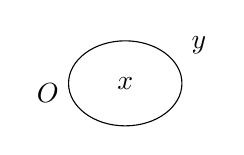
\begin{tikzpicture}[scale=0.6]
\draw (0,0) ellipse (1.2 and 0.9);\node at (0,0) {$x$};\node[left] at (-1.2,-0.2) {$O$};\node[right] at (1.2,0.8) {$y$};
\end{tikzpicture}
\end{adjustbox}
$x$ -- внутри, $y$ -- снаружи (в зад. конфиг.)
Гиббс. мера -- такая мера, что:
\begin{equation*}
\frac{d\mu(x_0\mid y)}{d\mu_0(x)}=\frac1{\Xi(y;O)}
e^{-[\sum_{x_i\in X}U_1(x_i)+\sum_{(x_i,x_j)\in X}U_2(x_i,x_j)+\sum_{\substack{x_i\in X\\y_j\in Y}}U_2(x_i,y_j)]}.
\end{equation*}
$x=(x_1,\ldots,x_k)$.
\begin{equation*}
X=\{X_0=X\cap O,\ Y=X\setminus X_0\}.
\end{equation*}
Всё это зависит только от $r_0$-окрестности $O$ (от тех точек $y$, к-рые туда попали).
$\mu(x\mid y)$ -- мера на конфигур. в $O$.
$\mu_0(x)$ -- мера -- [знак повтора] -- $O$.
(В опред. (1) подразумевается,
[зачеркнуто: \Incomplete{GELFAND-P000587}{definition-cancelled-clause}{Начало зачёркнутой фразы между «подразумевается» и «что» не прочитано полностью.} разн. частиц в разн. областях)]
что берётся $\sigma$-алг., порожд. соотв. цилиндрич. мн-вами.)
[Г. $\mu(x\mid y)$ опр., т.к. есть измеримое разбиение (теорема Фубини -- общая).
Мера на $Y$ индуцируется мерой всюду -- с пом. прообразов.]
Пусть есть 2 области.
\begin{adjustbox}{max width=\linewidth}
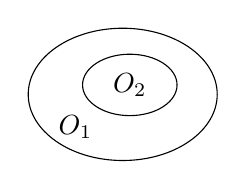
\begin{tikzpicture}[scale=0.6]
\draw (0,0) ellipse (2 and 1.4);\draw (0.15,0.2) ellipse (1 and 0.65);\node at (0.15,0.2) {$O_2$};\node at (-1,-0.7) {$O_1$};
\end{tikzpicture}
\end{adjustbox}
По мере $\mu$ на $X$ строится мера на $Y$ (дополним всеми возм. способами мн-вом $X_0$).

\SourcePage{GELFAND-P000588}{unlabelled}
\begin{adjustbox}{max width=\linewidth}
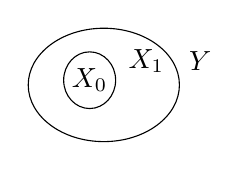
\begin{tikzpicture}[scale=0.6]
\draw (0,0) ellipse (1.6 and 1.2);\draw (-0.3,0.1) ellipse (0.55 and 0.6);\node at (-0.3,0.1) {$X_0$};\node at (0.9,0.5) {$X_1$};\node[right] at (1.6,0.5) {$Y$};
\end{tikzpicture}
\end{adjustbox}
Зафиксируем $X_0,X_1$ и $Y$. Тогда мера (усл.) вычисл. двумя способами:
\underline{Теорема.} [Зачеркнуто: \Incomplete{GELFAND-P000588}{existence-cancelled-mark}{Короткий знак перед существованием не прочитан.}]
$\exists$ хотя бы одно распред. Гиббса.
\underline{Док-во.}
\begin{adjustbox}{max width=\linewidth}
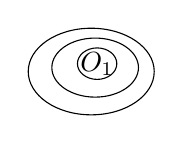
\begin{tikzpicture}[scale=0.5]
\draw (0,0) ellipse (1.6 and 1.1);\draw (0.1,0.1) ellipse (1.1 and 0.75);\draw (0.15,0.2) ellipse (0.5 and 0.4);\node at (0.15,0.2) {$O_1$};
\end{tikzpicture}
\end{adjustbox}
$O_1\subset O_2\subset O_3\subset\ldots$ и гран. условия зафиксир.
[Зачеркнуто: «Пусть».]
Пр-во конфиг. в $O_1$ -- компактно. $\exists$ подпосл., им. предел.
И т.д. $\ldots$
\underline{Пр. 1} $M$ -- прямая, $m$ -- мера Лебега $\Rightarrow$ распр. Гиббса только одно.
\underline{Пр. 2} $M=\mathbb R^k$, $U_1\equiv0$, $m(O)\le c\ell(O)$ ($\ell$ -- лебегова мера).
При малом $c$ распред. Гиббса единственно.

\underline{Решётчатое распред. Гиббса.}
Рассм. решётку в $M=\mathbb Z^d$, $d\ge2$.
\SourceFigure{GELFAND-P000588}{lattice-points}{Координатные оси с отмеченными узлами решётки, часть узлов -- точки, часть -- крестики; округлая область O окружает четыре узла справа над горизонтальной осью. Точная роль различных знаков не подписана.}
$X$ -- беск. подмн-ва точек решётки, $\mathcal M$.
$\mu_0$ -- вер. того, что есть частица $\frac12$, нет частицы $\frac12$,
и независ. в разн. точках.
$O$ -- конечная область.
\begin{equation*}
\mu(X_0\mid Y)=\frac1{\Xi(Y,O)}
e^{-\beta[\sum_{x\in X_0}U_1(x)+\sum_{(x_i,x_j)\in O}U_2(x_i,x_j)+\sum U_2(x_i,y_j)]}.
\end{equation*}
$U_2$ тоже обр. в $0$ при больших $|x-y|$.
$U_1\equiv0$, $U_2$ -- мала $\Rightarrow$ одно распр. Гиббса
(возмущ., вероятн. совм. распр. независ. случ. величин).
$U_1(x)=\alpha$, $U_2(x_i,x_j)=$
[зачеркнуто: \Unclear{GELFAND-P000588}{cancelled-pair-formula}{$U_2(|x_i+x_j|)$? или $U_2(|x_i-x_j|)$?; знак между $x_i$ и $x_j$ перекрыт штрихами зачёркивания; возможны $+$ и $-$, вертикальные штрихи и скобки не установлены окончательно}]
$U_2(x_i-x_j)$, $U_2(-x)=U_2(x)$.

\underline{1. Основное периодическое состояние.}
$X$ -- периодич. конфигурация (повторение прямоуг.).
\begin{adjustbox}{max width=\linewidth}
\begin{tikzpicture}[scale=0.5]\draw (0,0) rectangle (2.2,1.3);\end{tikzpicture}
\end{adjustbox}
\begin{equation*}
H(X)=\sum_{x\in X}U_1(x)+\sum_{x,y\in X}U_2(x,y)
\qquad\text{(формальное выражение)}.
\end{equation*}
Пусть $X'$ непериодич. и отл. от $X$ в кон. числе мест. Напишем $H(X')$ (тоже формально).
Если $H(X')-H(X)\ge0$ $\forall X'$, то $X$ наз. основным состоянием.
[Подчёркнутое неравенство: «уже опред.»]
1) Пусть $(X_1,X_2,$ [зачеркнуто: \Incomplete{GELFAND-P000588}{ground-state-tuple-cancel}{Знак в списке состояний перед многоточием закрыт чернилами.}]
$\ldots,X_k)=G(U)$ -- набор основных периодич. состояний, соотв. $U$.

\SourcePage{GELFAND-P000589}{unlabelled}
\underline{2) Условие Пайерлса (невырожденность осн. состояний):}
(чтобы осн. сост. -- [зачеркнуто: \Incomplete{GELFAND-P000589}{peierls-initial-mark}{Один знак в пояснении не прочитан.}]
осн. вклад в $e^{-\beta H}$).
\begin{equation*}
H(X')-H(X)>\cdots
\end{equation*}
[Зачёркнутый заголовок: \Incomplete{GELFAND-P000589}{peierls-cancelled-heading}{Короткий заголовок перед «Пусть» густо зачёркнут.}]
Пусть $\bar X$ -- произв. конфигурация.
\SourceFigure{GELFAND-P000589}{boundary-square}{Прямоугольная рамка, внутри точка $\ell$; стрелка справа направлена в рамку.}
[Зачёркнутая подпись у стрелки: \Incomplete{GELFAND-P000589}{boundary-label-cancel}{Короткая подпись перекрыта штрихами и не прочитана.}]
$\ell$ наз. точкой границы $\bar X$, если в окрест. $\ell$ $\bar X$ не совп. ни с одной из осн. периодич.
Пусть $\forall$ конфиг. $X'$, отлич. от $X$ в кон. числе точек,
\underline{Усл. Пайерлса:}
[В неравенстве перед $\Gamma(X')$ зачёркнут множитель: \Incomplete{GELFAND-P000589}{peierls-cancelled-factor}{Обозначение множителя перекрыто чернилами.}]
\begin{equation*}
H(X')-H(X)\ge g\,\Gamma(X'),\qquad(g>0).
\end{equation*}
[$\Gamma(X')$: стрелка к подписи «число гр. точек в $X'$».]

Включим $U$ [снизу: «пара $U_1,U_2$»] в $(k-1)$-парам. сем-во
$U_{\mu_1,\ldots,\mu_{k-1}}$, $U_{0,\ldots,0}=U$.
(Есть $k$ осн. сост. -- здесь то же $k$.)
\begin{equation*}
G(U_{\mu_1,\ldots,\mu_{k-1}})\subseteq G(U)\quad\text{при малых }\mu.
\end{equation*}
(Осн. сост. могут только пропасть). Пусть возмущ. «лин. незав.».
Тогда $\exists\beta_0$, $\forall\beta>\beta_0$
\begin{equation*}
\exists\{\mu_1(\beta),\ldots,\mu_{k-1}(\beta)\}=\vec\mu
\end{equation*}
при к-ром есть $k$ распред. Гиббса. Через неё прох. $k$ кривых,
на к-рых $k-1$ распр. Гиббса, $C_k^2$-поверхностей,
на к-рых $(k-2)$ распр. Гиббса и т.д.
\SourceFigure{GELFAND-P000589}{parameter-sketch}{Три утолщённые оси со стрелками вверх, вправо и вниз-влево; под пересечением подпись $\mu$ со стрелкой над ней. По обе стороны расположены несколько наклонных коротких штрихов. Справа от верхней части вертикальной оси виден отдельный тонкий волнистый штрих. Группировка и точная форма этих штрихов не восстанавливаются.}
При сдвигах «как правило» получ. одно осн. состояние.
\underline{Невырожденность:} с измен. $\mu_1,\ldots,\mu_k$ есть
\Unclear{GELFAND-P000589}{ground-state-count}{[два исправленных знака перед «одно»]}
[вставлено: «вообще говоря»] одно осн. состояние,
на кривых $\le(k-1)$ и т.д.
Тогда то же будет для распред. Гиббса.
\underline{Вопрос Гельфанда:} распр. Гиббса в $p$-адич. случае.

\SourcePage{GELFAND-P000590}{unlabelled}
[Верхняя часть кадра без текста.]
\underline{3/III -- 75} \underline{Сем. Гельфанда.}
\underline{В. Н. Туловский.} \underline{WF.} $\Omega\subset\mathbb R^n$, $u\in\mathcal D'(\Omega)$.
$(x_0,\xi_0)\notin WF(u)$, если $(x_0,\xi_0)\in\Omega\times(\mathbb R^n\setminus0)$ и
из $\Phi'(x_0)=\xi_0$ следует, что
\begin{equation*}
|\langle u,\varphi e^{i\lambda\Phi}\rangle|\le C_N\lambda^{-N},\qquad\forall N
\end{equation*}
(линейность $\Phi$ не важна).
Пусть $\Omega\subset\mathbb R^n$, $\theta\in\mathbb R^N$,
$a(x,\theta)\in S^m_{1,0}(\Omega\times\mathbb R^N)$.
$\Phi$ -- фазовая ф-я.
\begin{equation*}
\langle A,u\rangle=\int a(x,\theta)e^{i\Phi(x,\theta)}
u(x)\,dx\,d\theta=
\end{equation*}
[Первый знак в $u(x)$: \Unclear{GELFAND-P000590}{oscillatory-integrand-overwrite}{$u$?; густо переписан, прежний слой не установлен}.]

\SourcePage{GELFAND-P000591}{unlabelled}
\begin{equation*}
=\lim_{\varepsilon\to0}\int a(x,\theta)e^{i\Phi(x,\theta)}u(x)\chi(\varepsilon\theta)\,dx\,d\theta.
\end{equation*}
\begin{adjustbox}{max width=\linewidth}
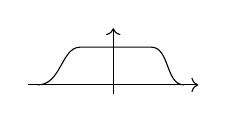
\begin{tikzpicture}[scale=0.6]
\draw[->] (-1.8,0)--(1.8,0);\draw[->] (0,-0.2)--(0,1.2);
\draw (-1.6,0)..controls(-1.1,0)and(-1.1,0.8)..(-0.7,0.8)--(0.8,0.8)..controls(1.2,0.8)and(1.1,0)..(1.5,0);
\end{tikzpicture}
\end{adjustbox}
Пусть $\Phi'_\theta(x_0,\theta_0)\ne0$. Напишем разложение $a=a_1+a_2$,
(\underline{пример:} $a=1$, $\Phi=\langle x,\theta\rangle$, $\langle A,u\rangle=u(0)$,
[зачеркнуто: \Incomplete{GELFAND-P000591}{delta-example-cancel}{Короткое слово перед «т.е.» не прочитано.}]
т.е. $A(x)=\delta(x)$).
Где $a_2$ сосред. в конич. окр. $(x_0,\theta_0)$,
а $a_1(x,\theta)=0$ в [зачеркнуто: \Incomplete{GELFAND-P000591}{amplitude-neighbourhood-cancel}{Слово после «в» густо зачёркнуто; ниже вставлено «точки».}]
окр. точки $(x_0,\theta_0)$.
\begin{equation*}
\langle A_2,u\rangle=\int a_2(x,\theta)e^{i\Phi(x,\theta)}u(x)\,dx\,d\theta,
\qquad\text{здесь }\Phi'_\theta\ne0\Rightarrow A_2\in C^\infty.
\end{equation*}
\begin{equation*}
C_\Phi=\{(x,\theta):\Phi'_\theta=0\}.
\end{equation*}
\underline{Теорема.} [Зачеркнуто: $WF$]
Рассм. отобр.
\begin{equation*}
\lambda_\Phi:C_\Phi\longrightarrow\Omega\times(\mathbb R^n\setminus0),
\qquad(x,\theta)\longrightarrow(x,\Phi'_x).
\end{equation*}
Обозначим: $\lambda_\Phi(C_\Phi)=\Lambda_\Phi$.
Тогда $WF(A)\subseteq\Lambda_\Phi$.
Невырожд. фазовые ф-и -- если $\operatorname{rank}(\Phi''_{\theta x},\Phi''_{\theta\theta})=N$ на $C_\Phi$.
Тогда $\lambda_\Phi$ -- лок. диффеом. и [зачеркнуто: \Incomplete{GELFAND-P000591}{before-lambda-cancel}{Короткий фрагмент перед обозначением Lambda перекрыт штрихами.}] $\Lambda_\Phi$ -- лагранжево конич. мн-зие,
т.е. $\langle\xi,dx\rangle|_{\Lambda_\Phi}=0$.
Обратно: $\forall$ конич. лагр. мн-зие локально можно получить из невыр. фазовой ф-и
(причём можно взять $N=n$).
[Зачеркнуто: «Пусть есть 2 невыр. фаз. ф-и.»
\Incomplete{GELFAND-P000591}{cancelled-phase-sentence-end}{Конец зачёркнутого предложения закрыт густой чертой.}]
Проверка лагранжевости:
\begin{equation*}
\Phi'_\theta(x,\theta)=0\Rightarrow\Phi(x,\theta)=0,
\end{equation*}
\begin{equation*}
\Phi'_\theta(x+dx,\theta+d\theta)=0,\quad
\Phi'_x\,dx+\underbrace{\Phi'_\theta\,d\theta}_{\text{«0»}}=0.
\end{equation*}
Отсюда $\Phi'_x\,dx=0$ на $\Lambda_\Phi$, или $\xi\,dx=0$ на $\Lambda_\Phi$. [Треугольный знак окончания.]
Пусть есть 2 фаз. ф-и $\Phi_1$ и $\Phi_2$,
$\lambda_{\Phi_1}:C_{\Phi_1}\to\Lambda$, $\lambda_{\Phi_2}:C_{\Phi_2}\to\Lambda$
($\Lambda$ одно и то же).
\begin{equation*}
(x_0,\theta_1^0)\longrightarrow(x_0,\xi_0),\qquad
(x_0,\theta_2^0)\longrightarrow(x_0,\xi_0).
\end{equation*}
Класс ф-й $A$ будет тот же для $\Phi_1$ и для $\Phi_2$.
\underline{ИОФ:} [Зачеркнуто: \Incomplete{GELFAND-P000591}{iof-intro-cancel}{Два густых перечёркнутых фрагмента перед обозначениями X и Y не прочитаны.}]
$X,Y$ -- 2 мн-зия, $\Lambda$ -- замкн. конич. лагр. мн-зие без особ. в $T^*(X\times Y)\setminus0$.
Тогда локально $\Lambda$ зад. с пом. фаз. ф-и $\Phi(x,y,\theta)$,
(в окр. [зачеркнуто: \Incomplete{GELFAND-P000591}{iof-point-cancel}{Один знак перед «точки» закрыт чернилами.}]
точки $(x_0,\xi_0,y_0,\eta_0)$), и выб. амплитуду $a$,
и опр. опер. с пом. ядра
\begin{equation*}
\int a(x,y,\theta)e^{i\Phi(x,y,\theta)}u(x,y)\,dx\,dy\,d\theta.
\end{equation*}
[Зачеркнуто: \Incomplete{GELFAND-P000591}{iof-final-cancel}{Малый фрагмент справа от последнего интеграла закрыт штрихами.}]

\SourcePage{GELFAND-P000592}{4}
\underline{Кириллов. Факт:} $M$ -- симпл. мн-зие, $\omega$ -- соотв. форма.
[Зачеркнуто: \Incomplete{GELFAND-P000592}{symplectic-form-cancel}{Короткий фрагмент после «форма» зачёркнут.}]
На $M$ есть \underline{лагранжево слоение}.
[Справа: пять параллельных открытых дуг.]
Тогда там есть на слоях инвар. опред. аффинная структура.
[Зачеркнуто: \Unclear{GELFAND-P000592}{before-if-cancelled-mark}{[один знак]}]
Если ф-и на $M$ постоянны на листах слоения, то их градиенты
(векторы, соотв. ковектору $d\varphi$) определяют там паралл. перенос.
Соотв. вект. поля коммутируют.
\begin{equation*}
\varphi\longrightarrow d\varphi\longrightarrow\xi_\varphi.
\end{equation*}
-- эти вект. поля [зачеркнуто: «коммутируют»] и наз. параллельными.
\underline{Следствие:} листы -- $\mathbb R^n$ или торы.
\Unclear{GELFAND-P000592}{framework-word}{Кокас.?} рассм. -- пример лагр. слоения.

\underline{Туловский.}
В общ. случае:
\begin{equation*}
\sum_j\int a_j(x,y,\theta_j)e^{i\Phi_j(x,y,\theta_j)}u(x,y)\,dx\,dy\,d\theta_j
\end{equation*}
-- это \underline{ИОФ}.
[Зачеркнуто: «Теорема».]
Это класс опер., для к-рых $WF(A)\subseteq\Lambda$ и \Unclear{GELFAND-P000592}{relative-clause-overwrite}{к-рые?; густо переписано, прежний слой не разделяется} хорошо действ. на быстро осцилл. exp.
Пусть $(x,\Psi'_x)$ трансверс. $\Lambda$.
\begin{equation*}
A(e^{it\Psi}\varphi)\sim e^{it\Phi}\sum_{j=0}^\infty b_j(x)t^{-\lambda_j}.
\end{equation*}
Тогда это ИОФ.
[Внизу: 4.]

\SourcePage{GELFAND-P000593}{unlabelled}
[Верхняя часть кадра без текста.]
\underline{10/III -- 75.} \underline{Сем. Гельфанда.}
\underline{Туловский.} (продолжение)
$\Omega_x\subseteq\mathbb R^{n_x}$, $\Omega_y\subseteq\mathbb R^{n_y}$.
\begin{equation*}
Au(x)=\int a(x,y,\theta)e^{i\Phi(x,y,\theta)}u(y)\,dy\,d\theta,
\qquad A:\mathcal E'(\Omega_y)\to\mathcal D'(\Omega_x).
\end{equation*}
С $\Phi$ ассоц. лагр. мн-зие $\Lambda\subset(\Omega_x\times\Omega_y)\times(\mathbb R^{n_x+n_y}\setminus0)$.
Случай ПДО: $\Lambda=(x,\xi,x,-\xi)$.
[Зачеркнуто: \Incomplete{GELFAND-P000593}{pdo-cancelled-notation}{Небольшая формула справа от случая ПДО не прочитана.}]
\underline{Вопрос Г.:} хорошо бы постр. в $p$-адич. случае.
Когда ядро $A(x,y)$ -- ядро ИОФ?
[Слева: \underline{отв. Туловского:}]
1) $WF(A)\subset\Lambda$ ($\Lambda$ -- нек-рое лагр. мн-зие).
2) $\forall\Psi:\{(x,\Psi'_x,y,\Psi'_y)\}$ трансвер. с $\Lambda\Rightarrow$
\begin{equation*}
\langle A,e^{it\Psi}\varphi(x,y)\rangle\sim\sum e^{it\widetilde\Psi}a_j(t,\ldots).
\end{equation*}
[Зачеркнуто: \Incomplete{GELFAND-P000593}{asymptotic-cancelled-clause}{Длинная строка под асимптотическим выражением густо перечёркнута.}]
и $\widetilde\Psi$ связано с $\Psi$ через $\Lambda$.
\underline{Т. 1.} $P(x,D_x)$ -- П.Д.О. 1-го пор. с вещ. ст. частью $p(x,\xi)$, $p(x_0,\xi_0)=0$,
$p'_{x,\xi}(x_0,\xi_0)\ne0\Rightarrow\exists2$ ИОФ
\begin{equation*}
A:\mathcal E'(\Omega_x)\to\mathcal E'(\mathbb R^n),\qquad
B:\mathcal E'(\mathbb R^n)\to\mathcal E'(\Omega_x),
\end{equation*}
\begin{equation*}
WF\left[P-B\frac{\partial}{\partial X_n}A\right]
\overset{/}{\ni}(x_0,\xi_0,x_0,-\xi_0).
\end{equation*}
[В первом $\xi_0$ зачёркнут или исправлен дополнительный знак:
\Unclear{GELFAND-P000593}{normal-form-covector-overwrite}{неразборчивый знак при $\xi_0$}.]
При этом
\begin{equation*}
WF(B\cdot A-I)
\overset{/}{\ni}(x_0,\xi_0;x_0,-\xi_0).
\end{equation*}
[В $B\cdot A$: \Unclear{GELFAND-P000593}{normal-form-operator-overwrite}{буквы, похожие на $B$ и $A$, густо переписаны; прежние штрихи не разделяются}.]
[Зачеркнуто: «Теорема».]
\underline{Т. 2} $P(x,D_x)u=f$
[зачеркнуто: \Incomplete{GELFAND-P000593}{equation-cancelled-mark}{Короткий знак после f закрыт штрихами.}],
\begin{equation*}
H_p=\sum\left(\frac{\partial p}{\partial x_j}\frac{\partial}{\partial\xi_j}
-\frac{\partial p}{\partial\xi_j}\frac{\partial}{\partial x_j}\right).
\end{equation*}
\begin{equation*}
WF(u)\setminus WF(f)\subset\{p(x,\xi)=0\}
\end{equation*}
и инвар. отн. гам. поля $H_p$.
След. раз Р. Л. Добрушин.
\SourcePage{GELFAND-P000594}{unlabelled}
\underline{И. Бернштейн.}

$WF$ левого ид. [зачёркнуто: \Unclear{GELFAND-P000594}{top-cancel}{опер.?}] дифф. опер. с полин. коэфф.
\begin{equation*}
=\{(x_0,\xi_0):\ \text{[переписанный знак]}\ p(x_0,\xi_0)=0,\ \forall p\}.
\end{equation*}
\Unclear{GELFAND-P000594}{top-quantifier}{переписанный знак, возможно $\forall$ или $\exists$.}
\underline{Теор.} $\dim WF\geq\dim X$.

\SourcePage{GELFAND-P000595}{unlabelled}
[Верхняя часть кадра без текста.]

\underline{\underline{17/III-75.}} \underline{Сем. Гельфанда.}

\underline{Программа семинара:}

\underline{\underline{Добрушин Р. Л.}}

Объекты

1) \underline{случ. поля с дискр. аргументом}

$X$ — [зачёркнуто: \Unclear{GELFAND-P000595}{middle-cancel-x}{изм. пр-во?}] конечное мн-во

$T$ — счётное мн-во
\begin{equation*}
X^T=(x_t,\ t\in T)
\end{equation*}
Случайное поле — вер. мера на $X^T$.

Физ. интерпр. — спиновые системы

2) \underline{точечные случ. поля}

$T$ — непр. пр-во $R^\nu$

Реализ. — [зачёркнуто: \Unclear{GELFAND-P000595}{lower-cancel-realiz}{конечные?}] подмн-ва $R^\nu$, $\cap$ к-рых с $\forall$ кон. объёмом конечно.

Мера на реализациях — точечное случ. поле.

3) $X(t),\quad t\in R^\nu\qquad S^*(R^\nu)$

[Стрелка от $X(t)$ вниз к:] ф-и (действ.)

случ. поле — мера на $S^*$

$\Rightarrow$ кв. теория поля.

\SourcePage{GELFAND-P000596}{unlabelled}
\underline{Проблема:} описание случ. полей
\begin{equation*}
T=Z,\quad X^Z\ (x_t,\ t\in Z)
\end{equation*}
\underline{\underline{Def}}
\begin{equation*}
\Pr(x_n\mid x_k,\ k\leq n)=\Pr(x_n\mid x_{n-1})\quad\text{(цепь Маркова)}
\end{equation*}
[Под левой условной вероятностью, со стрелкой вверх:] \underline{\underline{Усл. вер.}} известно.

[Под правой частью, с отметкой вверх:] \underline{марковский}

\Unclear{GELFAND-P000596}{upper-markov-index}{В условии слева написано $k\leq n$.}

\underline{Задание:} сначала зад. усл. вероятность и потом смотрим,
какие меры имеют эти усл. вероятности.

[Разделительная черта с точкой.]
\begin{equation*}
V\subset Z^\nu,\quad\text{зададим}\quad
\Pr\{\xi_n,\ n\in V\mid\xi_k,\ k\in Z^\nu\setminus V\}.
\end{equation*}
[Разделительная черта с точкой.]

Усл. вероятность: $(X,\mathcal B,\mu)$ — вероятн. пр-во.
\begin{equation*}
\mu(A\mid B)=\frac{\mu(A\cap B)}{\mu(B)}\quad\text{— недостаточно}
\end{equation*}
Пусть $\widetilde{\mathcal B}$ — подалгебра в $\mathcal B$

Усл. вероятность — [зачёркнуто: \Unclear{GELFAND-P000596}{middle-cancel-kernel}{ф-я?}; над строкой в обводке вставлено: мера] на [зачёркнуто: \Unclear{GELFAND-P000596}{middle-cancel-b}{неразборчивый знак перед $\mathcal B$}] $\mathcal B$, завис. от $x\in X$
\begin{equation*}
\mu(\cdot\mid x),\quad x\in X.
\end{equation*}
[Справа:] $\mu(B\mid x),\ B\in\mathcal B,\ x\in X.$

1) $\forall B:\ \mu(B\mid x)$ измерима на $\widetilde{\mathcal B}$

2)
\begin{equation*}
\int\psi(x)\varphi(x)\mu(dx)=\int\psi(x)\mu(dx\mid y)\varphi(y)\mu(dy)
\end{equation*}
$(\varphi$ измерима отн. $\widetilde{\mathcal B})$

Тогда соотв. $\mu$ и наз. усл. распр. вероятностей.

В широком классе случ. $\exists$ и единств.

\SourceFigure{GELFAND-P000596}{lower-strips}{Прямоугольник с рядом почти вертикальных отрезков. На среднем отрезке тёмная отметка и пересекающиеся штрихи. От этой области проведена линия вправо с видимым правым наконечником рядом с текстом «здесь мера…»; точная форма центральной отметки неясна.}

[Справа над подписью:] $\mu(B\mid x)$

здесь мера [малый указатель вверх к $\mu(B\mid x)$] сидит на отрезке.

Надо брать борелевские мн-ва (а не изм. по Лебегу)

В этом примере:
\begin{equation*}
\int\psi(x_1,x_2)\varphi(x_2)\,dx_1\,dx_2
=\int\left(\int\psi(x_1,x_2)\,dx_1\right)\varphi(x_2)\,dx_2
\end{equation*}
\begin{equation*}
P(B\mid\{\xi_\alpha,\alpha\in A\}).\qquad
P_{\mathcal B(\xi_\alpha,\alpha\in A)}(B\mid X)
\end{equation*}
\begin{equation*}
\xi_\alpha:X\to F_\alpha\quad\text{или одна}\quad\xi:X\to F\quad\text{(в прямое произв.)}
\end{equation*}
[Под $\xi_\alpha$, со стрелкой:] ф-и

[Под $F$:] точки $F$ — слои

прообразы мн-в в $F$ — $\widetilde{\mathcal B}$

[Со стрелкой от этой строки вниз:] там $\sigma$-алг. $\mathcal B_F$.

[Разделительная черта с точкой.]

\SourcePage{GELFAND-P000597}{unlabelled}
[Верхняя часть кадра без текста.]

\underline{Сем. Гельфанда.} \underline{31/III-75г.}

\underline{Поляков} (Саша) \underline{Об идее [вставлено над строкой в обводке: спонтанно] нарушенных симметрий}

«Пузырьки в эфире кв. теор. поля — частицы»

Skyrme; Нильсен, Ольсен, Фаддеев, Поляков, Хуфт.

\underline{Следующий раз} — теория Неванлинны (по Гриффитсу)

\SourcePage{GELFAND-P000598}{unlabelled}
\underline{7/IV-75.} \underline{Сем. Гельфанда.}

\underline{King} (?) \underline{Теория Неванлинны по Гриффитсу.}

\underline{2 идеи.} 1) hyperbolic analysis
\begin{equation*}
f:X\to V\qquad\text{negatively curved}
\end{equation*}
[Под $f$:] holomorphic

$\Rightarrow$ there are some restr. on behaviour of $f$.

2) ``counting'' of volume of divisors of analytic sets by
residue calculus.

\underline{Сначала 2)}

$g$ — голом. ф-я, $D=\{g^{-1}(0)\}$

\SourceFigure{GELFAND-P000598}{margin-contour}{На левом поле почти вертикальная линия, вокруг неё два дугообразных петлеобразных штриха. Их направление и точное замыкание неясны.}

интеграл по окр. от формы (меньшего порядка).

Пусть $\eta$ — любая форма степ. $r$ на $C^n\setminus D$

[Над строкой в обводке, со стрелкой к строке:] $\leftarrow$ это тоже форма
\begin{equation*}
\eta=\frac{dg}{2\pi ig}\wedge\zeta+\xi,\qquad
\zeta,\xi\text{ — формы, [зачёркнуто; остаток «то»?]}
\end{equation*}
\Unclear{GELFAND-P000598}{upper-type-cancel}{зачёркнутые штрихи и остаток «то»?}
\begin{equation*}
\lim_{\varepsilon\to0}\int_{C(\varepsilon)}\eta=\zeta|_D
\end{equation*}
[Зачёркнуто: \Unclear{GELFAND-P000598}{middle-cancel-flow}{неразборчивое короткое слово}] $\eta,\zeta$ — потоки (ф-и на формах): [зачёркнуто: так] их проще всего опр.:

[Под строкой:] (current)

\underline{Current:}
\begin{equation*}
T:A_c^k(V)\to C
\end{equation*}
\begin{equation*}
\lambda\in L_{loc}^1\ r\text{-form}\quad\Rightarrow\quad
[\lambda](\varphi)=\int_X\lambda\wedge\varphi,
\end{equation*}
\begin{equation*}
dT(\varphi)=\pm T(d\varphi).
\end{equation*}
Форма $\zeta|_D$ опр. поток:
\begin{equation*}
[\zeta|_D](\varphi)=\int\zeta\wedge\varphi.
\end{equation*}
\underline{Опр.} Пусть $\eta$ — $L_{loc}^1$-форма, $\in C^\infty$ на [над строкой: \Unclear{GELFAND-P000598}{middle-open-set}{обозначение $D_0$ или $D$}] открытом плотном мн-ве
\begin{equation*}
\operatorname{Res}\eta=[\zeta|_D]:=d[\eta]-[d\eta]
\end{equation*}
[Справа под обведённой строкой:] $\eta$ — обычная форма

[Зачёркнуто: \Unclear{GELFAND-P000598}{middle-cancel-normal}{(на ...; остальная часть неразборчива)}]

[Волнистая разделительная линия.]
\begin{equation*}
\begin{aligned}
d[\eta](\varphi)&\underset{def}{=}[\eta](d\varphi)=\int_V\eta\wedge d\varphi
=\lim_{\varepsilon\to0}\int_{V-U_\varepsilon(D)}\eta\wedge d\varphi=\\
&=\int_V d\eta\wedge\varphi-\lim_{\varepsilon\to0}\int_{\partial U_\varepsilon(D)}
=\int_V d\eta\wedge\varphi-\int_D\ldots
\end{aligned}
\end{equation*}
\underline{Пример:}
\begin{equation*}
\eta=\frac{dz}{z},\qquad [\eta](\varphi)=\int\frac{dz\wedge\varphi}{z}
\end{equation*}
\begin{equation*}
d[\eta](\varphi)-[\eta](d\varphi)
=\lim_{\varepsilon\to0}\int_{\text{[переписанный знак]}}\varphi\,dz=\varphi(0).
\end{equation*}
\Unclear{GELFAND-P000598}{lower-contour}{переписанный круглый знак, возможно $O$.}
\underline{$\operatorname{Res}\eta$ — поток.!}

$g$ — голом. ф-я на $\bar V$.

\Unclear{GELFAND-P000598}{lower-vbar}{Над $V$ отдельный длинный штрих; прочитано как черта.}
\begin{equation*}
\Rightarrow\quad\operatorname{Res}\left[\frac{dg}{2\pi ig}\right]=[Z],
\end{equation*}
\begin{equation*}
Z=\{g=0\},\quad Z=\bigcup Z_i,\quad\operatorname{ord}g=m_i\ \text{[переписано «на»?]}\ Z_i
\end{equation*}
\Unclear{GELFAND-P000598}{lower-order}{переписано «на»?}
\begin{equation*}
Z=\sum m_i\int_{Z_i}\qquad\text{(как поток)}
\end{equation*}

\SourcePage{GELFAND-P000599}{unlabelled}
Пусть $X\subset V$; $\operatorname{Codim}X=1$.
\begin{equation*}
X\cap U_i=\{g_i=0\}\qquad f_{ij}=\frac{g_i}{g_j}\text{ в }U_i\cap U_j
\end{equation*}
\begin{equation*}
\begin{adjustbox}{max width=\linewidth}
\begin{tikzcd} L_X\arrow[d]\\V\end{tikzcd}
\end{adjustbox}
\qquad\sigma=\{g_i\},\quad\sigma\in\Gamma(L_X).
\end{equation*}
$\sigma=0$ на $X$.

[Разделительная черта с точкой.]

Пусть на $L$ есть эрм. метрика ($L$ — 1-мерн. расслоение)

Можно рассм. $|\sigma|^2\in C^\infty$ на $V$ и $=0$ на $X$.
\begin{equation*}
\eta=\frac{1}{2\pi i}\partial\log|\sigma|^2,\qquad
\partial\log|z|^2=\frac{dz}{z}.
\end{equation*}
Тогда $\operatorname{Res}\eta=[X]$.
\begin{equation*}
[d\eta]=\frac{\bar\partial\partial}{2\pi i}\log|\sigma|^2
=\frac{\bar\partial\partial}{2\pi i}\log h_i=c(L_D).
\end{equation*}
[Справа:] \underline{(класс Черна)}

где $|\sigma|^2=h_i|g_i|^2$
\begin{equation*}
\partial\bar\partial\log\bar g_i=0
\end{equation*}
\Unclear{GELFAND-P000599}{upper-log-conjugate}{В отдельной строке видны черты над вторым $\partial$ и над $g_i$.}

Теор. де Рама выполняется! (в потоки):
\begin{equation*}
\underline{X=d[\eta]+[c(L_D)]}
\end{equation*}
(класс Черна когомологичен мн-ву нулей любого сечения)!

[Разделительная черта с точкой.]

Пусть $\psi$ — замкн. форма. [Вставлено над строкой в обводке: Тогда]
\begin{equation*}
\int_X\psi=\int_V c(L_D)\wedge\psi.
\end{equation*}
\underline{Теоремы типа Безу.} Пусть $X,Y$ [зачёркнуто: \Unclear{GELFAND-P000599}{middle-xy-cancel}{плотный знак, похожий на решётку}] — две кривые в $CP^2$.
\begin{equation*}
X=d[\eta_X]+\varphi_X
\end{equation*}
\begin{equation*}
Y=d[\eta_Y]+\varphi_Y
\end{equation*}
[Справа:] $(\varphi_X$ — кл. Черна)

[Зачёркнуто: \Unclear{GELFAND-P000599}{middle-phi-cancel}{малый знак перед «для»}] для $X$ — $[c(L_D)]$

Рассмотрим
\begin{equation*}
\int_V\varphi_X\wedge\varphi_Y=\int_X\varphi_Y=[X\wedge Y](1)
\end{equation*}
(число точек пересеч. $=$ произв. классов Черна)

\underline{Пример:} $V=P^2,\quad X,Y=H$ (гиперпл.)
\begin{equation*}
d_X=\operatorname{deg}X=\#(X\cap H)=\int_X\omega
\end{equation*}
($\omega$ — станд. форма, двойств. гиперпл. сеч.)
\begin{equation*}
\varphi_X=X\sim\ \text{[малый знак над строкой]}
\end{equation*}
\Unclear{GELFAND-P000599}{lower-equivalence}{малый знак над строкой после $\sim$, похожий на уголок.}
\begin{equation*}
\int_{P^2}\varphi_X\wedge\varphi_Y=d_Xd_Y\int_{P^2}\omega^2=d_X\cdot d_Y
\end{equation*}
— это док-во теор. Безу о числе точек пересеч. кривых.

\SourcePage{GELFAND-P000600}{unlabelled}
\underline{$X$ с особенностями} $\Rightarrow$ \underline{теор. сохраняется} (Lelong, 1953)

[Разделительная черта с точкой.]

\underline{1) idea.}
\begin{equation*}
f:C^n\overset{\text{holom.}}{\longrightarrow}V
\end{equation*}
[Под $C^n$:] $\varphi\leftarrow$ евкл. кэлер.

[Стрелка к $V$:] compact. Kaehler ([вставлено над строкой в обводке: with] form $\omega$).

Пусть $B(r)$ — шар рад. $r$.
\begin{equation*}
\operatorname{vol}(f(B(r)))=\int_{B(r)}f^*(\omega^n)
\end{equation*}
\SourceFigure{GELFAND-P000600}{upper-graph}{Оси с общим началом: вертикальная подписана $C^n$ и имеет наконечник вверх, горизонтальная подписана $V$. Правый конец горизонтальной оси слегка утолщён и заострён вправо, возможно наконечник. Из начала идёт вверх и вправо волнистая линия. Точная связь этой схемы с обозначением графика справа требует проверки; дополнительных точек нет.}

[Справа:] \Unclear{GELFAND-P000600}{upper-graph-label}{плотно переписанное $\Gamma$ с индексом, возможно $f$ или $r$} [вставлено над строкой в обводке: часть] графика $f$. над $B(r)$
\begin{equation*}
\int_{\Gamma(r)}(\varphi+\omega)^n
=\sum\binom nk\int_{B(r)}\varphi^k\wedge f^*\omega^{n-k}
\end{equation*}
\underline{\underline{Опрд.}}
\begin{equation*}
T_k(f,r)\underset{def}{=}\int_{B(r)}\varphi^{n-k}\wedge f^*(\omega^k)
\end{equation*}
[Волнистая разделительная линия.]

Во мн. случаях $T_k=O(T_1)$ (по $r$ — рост).

[Под строкой:] одного порядка.
\begin{equation*}
\begin{adjustbox}{max width=\linewidth}
\begin{tikzcd}
& L\arrow[d]\\
C^n\arrow[r,"f"]&V
\end{tikzcd}
\end{adjustbox}
\end{equation*}
[Стрелка к $L$:] holom. line bundle.

Пусть $0<\omega=c(L)$ — его класс Черна

Пусть $\sigma\in O(L),\quad D=\{\sigma=0\}$.
\begin{equation*}
d[\eta]-[\omega]=[D];\qquad D_f=f^{-1}D.
\end{equation*}
\begin{equation*}
d[f^*\eta]-[f^*\omega]=[f^{-1}D]\quad\text{(на }C^n\text{).}
\end{equation*}
Умн. на $\chi_{B(r)}\varphi^{n-1}$:
\begin{equation*}
\underbrace{\int_{\text{[}S(r)\text{?]}}\varphi^{n-1}\wedge f^*\omega}_{\text{``}T_1}
=\int_{D_f}\chi_{B(r)}\varphi^{n-1}
\end{equation*}
\Unclear{GELFAND-P000600}{lower-count-domain}{$S(r)$?}
\begin{equation*}
\eta=\underbrace{\frac1{4\pi}\ \text{[зачёркнутый знак]}\ (\bar\partial-\partial)}_{d^c}\log|\sigma|^2.
\end{equation*}
\Unclear{GELFAND-P000600}{lower-eta-cancel}{зачёркнутый знак, возможно $i$.}
\begin{equation*}
\int_{D_f\cap B(r)}\varphi^{n-1}
\end{equation*}
(объём мн-ва нулей; \Unclear{GELFAND-P000600}{lower-volume-word}{помер. или номер.} с пом. станд. $\varphi$).
\begin{equation*}
T_1=\int_0^r\frac{t_1(f,\rho)}\rho\,d\rho
\end{equation*}
— $t_1\leftrightarrow T_1$ в обычн. теор. Неванлинны.

\SourcePage{GELFAND-P000601}{unlabelled}
[Зачёркнуто: \Unclear{GELFAND-P000601}{top-cancel-count}{начало формулы $N(\ldots)$, густо заштрихованное}]
\begin{equation*}
N(D_f,r)=\int_0^r\frac{\displaystyle\int_{D_f\cap B(\rho)}\varphi^{n-1}}{\rho^{n+1}}\,d\rho
\end{equation*}
\begin{equation*}
N(D_f,r)\leq T(f,r)+O(1)\qquad\text{(1-е нер-во Неванлинны)}
\end{equation*}
[Остальная часть кадра без текста.]

\SourcePage{GELFAND-P000602}{unlabelled}
\underline{14/IV-75.} \underline{Сем. Гельфанда.} \underline{King} (продолжение).
\begin{equation*}
C^n\overset f\longrightarrow V^n,\qquad D\subset V^n,\qquad D\sim c(L_D)=\omega
\end{equation*}
[Под $V^n$:] проект.

[Под $D$:] дивизор.

[Под $\omega$:] кэлер. форма
\begin{equation*}
N(D_f,r)\leq T(f,r)
\end{equation*}
[Под $N$:] объём прообраза дивизора (``число нулей'')

[Под $T$:] $\displaystyle\int_0^r\int_{B(r)} f^*\omega\wedge\psi^{n-1}\frac{dt}t$

(``порядок роста'')

[Справа:] (1-я теор. Неванлинны — трив.)

\underline{использ. теор. вычетов.}
\begin{equation*}
\operatorname{Ric}\Omega=i\partial\bar\partial\log g
\quad\Leftarrow\quad
\left(\Omega=\frac i2g\,dz\wedge d\bar z\right).
\end{equation*}
(тензор Риччи).
\begin{equation*}
\underline{n=1}\quad\Rightarrow\quad\operatorname{Ric}\Omega=k\Omega
\quad\text{(}\underline{k=\text{ — gaussian curvature}}\text{)}
\end{equation*}
\Unclear{GELFAND-P000602}{upper-gaussian-dash}{После $k=$ виден отдельный длинный горизонтальный штрих: тире или минус.}

$\Omega$ — $(n,n)$-форма объёма

[Справа:] $a(\cdot)\,dz_1\,d\bar z_1\ldots dz_n\,d\bar z_n$
\begin{equation*}
\operatorname{Ric}\Omega=\frac i{2\pi}\partial\bar\partial\log a
\end{equation*}
1) $\operatorname{Ric}\Omega>0$

2) $(\operatorname{Ric}\Omega)^n\geq\Omega$ (vol. form).

\underline{Ahlfors Lemma.}

Пусть $B^n$ или $\Delta^n$ имеет Бергмана-форму с крив. \Unclear{GELFAND-P000602}{middle-curvature-cancel}{густо переписанный знак, похожий на $H$ или $K$} $-1$
\begin{equation*}
\Rightarrow\ \forall\text{ голом. }f:B^n\to\text{[переписанная буква]}^{n};
\quad\Omega_V\text{ — форма объёма с отр. крив.}
\end{equation*}
\Unclear{GELFAND-P000602}{middle-target}{переписанная буква, возможно $V$.}
\begin{equation*}
f^*\Omega_V\leq\Phi_B\text{ — форма объёма}
\end{equation*}
[Разделительная черта с точкой, продолженная штрихами.]

[Зачёркнуто: Acta] \underline{Acta Math.; Griffits, King,} [зачёркнуто: \Unclear{GELFAND-P000602}{lower-final-cancel}{малый плотный знак, возможно $a$}]

\Unclear{GELFAND-P000602}{lower-name}{Heuman или Herman; знак связи похож на $>$ или $\Rightarrow$} Joachim Weil

Неприв. формулир. нужна в теории соб. ф-й.

Griffits, Cowen

\end{document}
